% Options for packages loaded elsewhere
\PassOptionsToPackage{unicode}{hyperref}
\PassOptionsToPackage{hyphens}{url}
\documentclass[
  english,
]{article}
\usepackage{xcolor}
\usepackage[margin=1in]{geometry}
\usepackage{amsmath,amssymb}
\setcounter{secnumdepth}{-\maxdimen} % remove section numbering
\usepackage{iftex}
\ifPDFTeX
  \usepackage[T1]{fontenc}
  \usepackage[utf8]{inputenc}
  \usepackage{textcomp} % provide euro and other symbols
\else % if luatex or xetex
  \usepackage{unicode-math} % this also loads fontspec
  \defaultfontfeatures{Scale=MatchLowercase}
  \defaultfontfeatures[\rmfamily]{Ligatures=TeX,Scale=1}
\fi
\usepackage{lmodern}
\ifPDFTeX\else
  % xetex/luatex font selection
\fi
% Use upquote if available, for straight quotes in verbatim environments
\IfFileExists{upquote.sty}{\usepackage{upquote}}{}
\IfFileExists{microtype.sty}{% use microtype if available
  \usepackage[]{microtype}
  \UseMicrotypeSet[protrusion]{basicmath} % disable protrusion for tt fonts
}{}
\makeatletter
\@ifundefined{KOMAClassName}{% if non-KOMA class
  \IfFileExists{parskip.sty}{%
    \usepackage{parskip}
  }{% else
    \setlength{\parindent}{0pt}
    \setlength{\parskip}{6pt plus 2pt minus 1pt}}
}{% if KOMA class
  \KOMAoptions{parskip=half}}
\makeatother
\usepackage{color}
\usepackage{fancyvrb}
\newcommand{\VerbBar}{|}
\newcommand{\VERB}{\Verb[commandchars=\\\{\}]}
\DefineVerbatimEnvironment{Highlighting}{Verbatim}{commandchars=\\\{\}}
% Add ',fontsize=\small' for more characters per line
\usepackage{framed}
\definecolor{shadecolor}{RGB}{248,248,248}
\newenvironment{Shaded}{\begin{snugshade}}{\end{snugshade}}
\newcommand{\AlertTok}[1]{\textcolor[rgb]{0.94,0.16,0.16}{#1}}
\newcommand{\AnnotationTok}[1]{\textcolor[rgb]{0.56,0.35,0.01}{\textbf{\textit{#1}}}}
\newcommand{\AttributeTok}[1]{\textcolor[rgb]{0.13,0.29,0.53}{#1}}
\newcommand{\BaseNTok}[1]{\textcolor[rgb]{0.00,0.00,0.81}{#1}}
\newcommand{\BuiltInTok}[1]{#1}
\newcommand{\CharTok}[1]{\textcolor[rgb]{0.31,0.60,0.02}{#1}}
\newcommand{\CommentTok}[1]{\textcolor[rgb]{0.56,0.35,0.01}{\textit{#1}}}
\newcommand{\CommentVarTok}[1]{\textcolor[rgb]{0.56,0.35,0.01}{\textbf{\textit{#1}}}}
\newcommand{\ConstantTok}[1]{\textcolor[rgb]{0.56,0.35,0.01}{#1}}
\newcommand{\ControlFlowTok}[1]{\textcolor[rgb]{0.13,0.29,0.53}{\textbf{#1}}}
\newcommand{\DataTypeTok}[1]{\textcolor[rgb]{0.13,0.29,0.53}{#1}}
\newcommand{\DecValTok}[1]{\textcolor[rgb]{0.00,0.00,0.81}{#1}}
\newcommand{\DocumentationTok}[1]{\textcolor[rgb]{0.56,0.35,0.01}{\textbf{\textit{#1}}}}
\newcommand{\ErrorTok}[1]{\textcolor[rgb]{0.64,0.00,0.00}{\textbf{#1}}}
\newcommand{\ExtensionTok}[1]{#1}
\newcommand{\FloatTok}[1]{\textcolor[rgb]{0.00,0.00,0.81}{#1}}
\newcommand{\FunctionTok}[1]{\textcolor[rgb]{0.13,0.29,0.53}{\textbf{#1}}}
\newcommand{\ImportTok}[1]{#1}
\newcommand{\InformationTok}[1]{\textcolor[rgb]{0.56,0.35,0.01}{\textbf{\textit{#1}}}}
\newcommand{\KeywordTok}[1]{\textcolor[rgb]{0.13,0.29,0.53}{\textbf{#1}}}
\newcommand{\NormalTok}[1]{#1}
\newcommand{\OperatorTok}[1]{\textcolor[rgb]{0.81,0.36,0.00}{\textbf{#1}}}
\newcommand{\OtherTok}[1]{\textcolor[rgb]{0.56,0.35,0.01}{#1}}
\newcommand{\PreprocessorTok}[1]{\textcolor[rgb]{0.56,0.35,0.01}{\textit{#1}}}
\newcommand{\RegionMarkerTok}[1]{#1}
\newcommand{\SpecialCharTok}[1]{\textcolor[rgb]{0.81,0.36,0.00}{\textbf{#1}}}
\newcommand{\SpecialStringTok}[1]{\textcolor[rgb]{0.31,0.60,0.02}{#1}}
\newcommand{\StringTok}[1]{\textcolor[rgb]{0.31,0.60,0.02}{#1}}
\newcommand{\VariableTok}[1]{\textcolor[rgb]{0.00,0.00,0.00}{#1}}
\newcommand{\VerbatimStringTok}[1]{\textcolor[rgb]{0.31,0.60,0.02}{#1}}
\newcommand{\WarningTok}[1]{\textcolor[rgb]{0.56,0.35,0.01}{\textbf{\textit{#1}}}}
\usepackage{longtable,booktabs,array}
\usepackage{caption}
\captionsetup[table]{skip=6pt}
\newcounter{none} % for unnumbered tables
\usepackage{calc} % for calculating minipage widths
% Correct order of tables after \paragraph or \subparagraph
\usepackage{etoolbox}
\makeatletter
\patchcmd\longtable{\par}{\if@noskipsec\mbox{}\fi\par}{}{}
\makeatother
\usepackage{graphicx}
\makeatletter
\newsavebox\pandoc@box
\newcommand*\pandocbounded[1]{% scales image to fit in text height/width
  \sbox\pandoc@box{#1}%
  \Gscale@div\@tempa{\textheight}{\dimexpr\ht\pandoc@box+\dp\pandoc@box\relax}%
  \Gscale@div\@tempb{\linewidth}{\wd\pandoc@box}%
  \ifdim\@tempb\p@<\@tempa\p@\let\@tempa\@tempb\fi% select the smaller of both
  \ifdim\@tempa\p@<\p@\scalebox{\@tempa}{\usebox\pandoc@box}%
  \else\usebox{\pandoc@box}%
  \fi%
}
% Set default figure placement to htbp
\def\fps@figure{htbp}
\makeatother
\ifLuaTeX
\usepackage[bidi=basic,shorthands=off]{babel}
\else
\usepackage[bidi=default,shorthands=off]{babel}
\fi
\ifLuaTeX
  \usepackage{selnolig} % disable illegal ligatures
\fi
\setlength{\emergencystretch}{3em} % prevent overfull lines
\providecommand{\tightlist}{%
  \setlength{\itemsep}{0pt}\setlength{\parskip}{0pt}}
\usepackage{bookmark}
\IfFileExists{xurl.sty}{\usepackage{xurl}}{} % add URL line breaks if available
\urlstyle{same}
% fallback for those not using the hyperref driver hyperxmp:
\makeatletter
\@ifundefined{xmpquote}{\newcommand{\xmpquote}[1]{#1}}{}
\makeatother
\hypersetup{
  pdftitle={From Distances to Maps: Multidimensional Scaling},
  pdfauthor={Livio Finos, University of Padova},
  pdflang={en},
  hidelinks,
  pdfcreator={LaTeX via pandoc}}

\title{From Distances to Maps: Multidimensional Scaling}
\usepackage{etoolbox}
\makeatletter
\providecommand{\subtitle}[1]{% add subtitle to \maketitle
  \apptocmd{\@title}{\par {\large #1 \par}}{}{}
}
\makeatother
\subtitle{Unit 11 --- Data Visualization}
\author{Livio Finos, University of Padova}
\date{}

\begin{document}
\maketitle

{
\setcounter{tocdepth}{3}
\tableofcontents
}
\section{Why work with distances?}\label{why-work-with-distances}

Many datasets are naturally represented as a rectangular table: one row
per person, site, product or image; one column per measured variable. In
other problems, the scientifically meaningful starting point is not a
variable but a \textbf{comparison between objects}. Examples include:

\begin{itemize}
\tightlist
\item
  ecological sites compared through their species composition;
\item
  products compared through consumer ratings or ingredient profiles;
\item
  patients compared through a set of symptoms or biomarkers;
\item
  cities compared through travel time rather than straight-line
  geography.
\end{itemize}

In all these cases we can ask the same question:

\begin{quote}
Which objects are close, which are far apart, and can that structure be
shown in a useful low-dimensional map?
\end{quote}

This unit introduces distances and \textbf{classical multidimensional
scaling (MDS)}. It deliberately concerns non-textual data. Text
documents will be treated later, when we can make the preprocessing and
weighting choices explicit.

\subsection{Learning goals}\label{learning-goals}

By the end of the unit, you should be able to:

\begin{itemize}
\tightlist
\item
  distinguish an object-by-variable table from an object-by-object
  distance matrix;
\item
  state the properties of a metric and recognise a dissimilarity that is
  not one;
\item
  calculate and compare Euclidean, Manhattan, Jaccard and Bray--Curtis
  distances;
\item
  explain why standardisation and the choice of distance are modelling
  decisions;
\item
  construct and interpret a classical MDS configuration in R;
\item
  connect the MDS construction to spectral decomposition;
\item
  use eigenvalues to diagnose whether a distance is exactly Euclidean
  and how well a two-dimensional map represents it.
\end{itemize}

\textbf{Prerequisites:} vectors and matrices, Euclidean distance,
centring, and the spectral decomposition of a real symmetric matrix. You
do not need prior knowledge of clustering or ordination.

\section{Objects, variables and distance
matrices}\label{objects-variables-and-distance-matrices}

Let \(x_i=(x_{i1},\ldots,x_{ip})\) denote the measurements for object
\(i\). After choosing a comparison rule \(d\), we obtain the distance
matrix

\[D=(d_{ij}),\qquad d_{ij}=d(x_i,x_j).\]

The matrix is square, symmetric and has zeros on its diagonal. It
contains \(n(n-1)/2\) distinct pairwise comparisons, not \(np\) original
measurements. This distinction matters: the original variables may
disappear after distances are computed, so their units and preprocessing
choices must be documented.

\begin{Shaded}
\begin{Highlighting}[]
\NormalTok{points3 }\OtherTok{\textless{}{-}} \FunctionTok{rbind}\NormalTok{(}\AttributeTok{A =} \FunctionTok{c}\NormalTok{(}\DecValTok{0}\NormalTok{, }\DecValTok{0}\NormalTok{), }\AttributeTok{B =} \FunctionTok{c}\NormalTok{(}\DecValTok{3}\NormalTok{, }\DecValTok{4}\NormalTok{), }\AttributeTok{C =} \FunctionTok{c}\NormalTok{(}\DecValTok{3}\NormalTok{, }\DecValTok{0}\NormalTok{))}
\NormalTok{points3}
\end{Highlighting}
\end{Shaded}

\begin{verbatim}
#>   [,1] [,2]
#> A    0    0
#> B    3    4
#> C    3    0
\end{verbatim}

\begin{Shaded}
\begin{Highlighting}[]
\FunctionTok{round}\NormalTok{(}\FunctionTok{as.matrix}\NormalTok{(}\FunctionTok{dist}\NormalTok{(points3)), }\DecValTok{2}\NormalTok{)}
\end{Highlighting}
\end{Shaded}

\begin{verbatim}
#>   A B C
#> A 0 5 3
#> B 5 0 4
#> C 3 4 0
\end{verbatim}

For these coordinates, \(d(A,B)=5\) under Euclidean distance. The matrix
says that A is farthest from B and that C lies between them in one
sense, but it no longer records that the original variables were
horizontal and vertical position.

\subsection{Metric or general
dissimilarity?}\label{metric-or-general-dissimilarity}

A \textbf{metric} satisfies, for every pair or triple of objects,

\[\begin{aligned}
d(x_i,x_j)&\geq 0 &&\text{(non-negativity)},\\
d(x_i,x_j)&=0 \Leftrightarrow x_i=x_j &&\text{(identity)},\\
d(x_i,x_j)&=d(x_j,x_i) &&\text{(symmetry)},\\
d(x_i,x_k)&\leq d(x_i,x_j)+d(x_j,x_k) &&\text{(triangle inequality)}.
\end{aligned}\]

In applications, we also use broader \textbf{dissimilarities}. They may
be useful even when one of these properties fails. For example, a
directed travel time may fail symmetry; a correlation-based
dissimilarity may not have a direct physical unit. The important
question is not whether a formula is fashionable, but whether it
expresses the scientific comparison we need.

\section{Four useful ways to compare
objects}\label{four-useful-ways-to-compare-objects}

\subsection{Euclidean distance: straight-line
difference}\label{euclidean-distance-straight-line-difference}

For quantitative variables on commensurate scales,

\[d_E(x_i,x_j)=\left\{\sum_{k=1}^p(x_{ik}-x_{jk})^2\right\}^{1/2}.\]

Euclidean distance gives large differences disproportionate influence
because they are squared. It is appropriate when the variables define
meaningful Cartesian coordinates, or when a straight-line geometry is
substantively useful.

\begin{Shaded}
\begin{Highlighting}[]
\NormalTok{pair\_index }\OtherTok{\textless{}{-}} \FunctionTok{combn}\NormalTok{(}\FunctionTok{seq\_len}\NormalTok{(}\FunctionTok{nrow}\NormalTok{(points3)), }\DecValTok{2}\NormalTok{)}
\NormalTok{euclidean\_calculations }\OtherTok{\textless{}{-}} \FunctionTok{apply}\NormalTok{(pair\_index, }\DecValTok{2}\NormalTok{, }\ControlFlowTok{function}\NormalTok{(index) \{}
\NormalTok{  first }\OtherTok{\textless{}{-}}\NormalTok{ points3[index[}\DecValTok{1}\NormalTok{], ]}
\NormalTok{  second }\OtherTok{\textless{}{-}}\NormalTok{ points3[index[}\DecValTok{2}\NormalTok{], ]}
  \FunctionTok{tibble}\NormalTok{(}
    \AttributeTok{pair =} \FunctionTok{paste}\NormalTok{(}\FunctionTok{rownames}\NormalTok{(points3)[index], }\AttributeTok{collapse =} \StringTok{"{-}{-}"}\NormalTok{),}
    \AttributeTok{calculation =} \FunctionTok{sprintf}\NormalTok{(}\StringTok{"sqrt((\%g {-} \%g)\^{}2 + (\%g {-} \%g)\^{}2)"}\NormalTok{,}
\NormalTok{                        first[}\DecValTok{1}\NormalTok{], second[}\DecValTok{1}\NormalTok{], first[}\DecValTok{2}\NormalTok{], second[}\DecValTok{2}\NormalTok{]),}
    \AttributeTok{distance =} \FunctionTok{sqrt}\NormalTok{(}\FunctionTok{sum}\NormalTok{((first }\SpecialCharTok{{-}}\NormalTok{ second)}\SpecialCharTok{\^{}}\DecValTok{2}\NormalTok{))}
\NormalTok{  )}
\NormalTok{\}) }\SpecialCharTok{|\textgreater{}} \FunctionTok{bind\_rows}\NormalTok{()}
\NormalTok{knitr}\SpecialCharTok{::}\FunctionTok{kable}\NormalTok{(euclidean\_calculations, }\AttributeTok{digits =} \DecValTok{2}\NormalTok{,}
             \AttributeTok{caption =} \StringTok{"Coordinate{-}by{-}coordinate Euclidean calculations."}\NormalTok{)}
\end{Highlighting}
\end{Shaded}

\begin{longtable}[]{@{}llr@{}}
\caption{Coordinate-by-coordinate Euclidean
calculations.}\tabularnewline
\toprule\noalign{}
pair & calculation & distance \\
\midrule\noalign{}
\endfirsthead
\toprule\noalign{}
pair & calculation & distance \\
\midrule\noalign{}
\endhead
\bottomrule\noalign{}
\endlastfoot
A--B & sqrt((0 - 3)\^{}2 + (0 - 4)\^{}2) & 5 \\
A--C & sqrt((0 - 3)\^{}2 + (0 - 0)\^{}2) & 3 \\
B--C & sqrt((3 - 3)\^{}2 + (4 - 0)\^{}2) & 4 \\
\end{longtable}

\begin{Shaded}
\begin{Highlighting}[]
\NormalTok{D\_euclidean\_points3 }\OtherTok{\textless{}{-}} \FunctionTok{matrix}\NormalTok{(}\DecValTok{0}\NormalTok{, }\FunctionTok{nrow}\NormalTok{(points3), }\FunctionTok{nrow}\NormalTok{(points3),}
                              \AttributeTok{dimnames =} \FunctionTok{list}\NormalTok{(}\FunctionTok{rownames}\NormalTok{(points3), }\FunctionTok{rownames}\NormalTok{(points3)))}
\ControlFlowTok{for}\NormalTok{ (i }\ControlFlowTok{in} \FunctionTok{seq\_len}\NormalTok{(}\FunctionTok{nrow}\NormalTok{(points3) }\SpecialCharTok{{-}} \DecValTok{1}\NormalTok{)) \{}
  \ControlFlowTok{for}\NormalTok{ (j }\ControlFlowTok{in}\NormalTok{ (i }\SpecialCharTok{+} \DecValTok{1}\NormalTok{)}\SpecialCharTok{:}\FunctionTok{nrow}\NormalTok{(points3)) \{}
\NormalTok{    D\_euclidean\_points3[i, j] }\OtherTok{\textless{}{-}}\NormalTok{ D\_euclidean\_points3[j, i] }\OtherTok{\textless{}{-}}
      \FunctionTok{sqrt}\NormalTok{(}\FunctionTok{sum}\NormalTok{((points3[i, ] }\SpecialCharTok{{-}}\NormalTok{ points3[j, ])}\SpecialCharTok{\^{}}\DecValTok{2}\NormalTok{))}
\NormalTok{  \}}
\NormalTok{\}}
\NormalTok{knitr}\SpecialCharTok{::}\FunctionTok{kable}\NormalTok{(D\_euclidean\_points3, }\AttributeTok{digits =} \DecValTok{2}\NormalTok{,}
             \AttributeTok{caption =} \StringTok{"Euclidean distance matrix, assembled from the displayed calculations."}\NormalTok{)}
\end{Highlighting}
\end{Shaded}

\begin{longtable}[]{@{}lrrr@{}}
\caption{Euclidean distance matrix, assembled from the displayed
calculations.}\tabularnewline
\toprule\noalign{}
& A & B & C \\
\midrule\noalign{}
\endfirsthead
\toprule\noalign{}
& A & B & C \\
\midrule\noalign{}
\endhead
\bottomrule\noalign{}
\endlastfoot
A & 0 & 5 & 3 \\
B & 5 & 0 & 4 \\
C & 3 & 4 & 0 \\
\end{longtable}

\subsection{Manhattan distance: total coordinate-wise
change}\label{manhattan-distance-total-coordinate-wise-change}

The Manhattan (or \(L_1\)) distance is

\[d_M(x_i,x_j)=\sum_{k=1}^p |x_{ik}-x_{jk}|.\]

It measures the total absolute difference and is less dominated by one
very large coordinate difference than Euclidean distance. It can be
motivated by movement along a grid, but it is also a general robust
alternative for numerical profiles.

\begin{Shaded}
\begin{Highlighting}[]
\NormalTok{manhattan\_calculations }\OtherTok{\textless{}{-}} \FunctionTok{apply}\NormalTok{(pair\_index, }\DecValTok{2}\NormalTok{, }\ControlFlowTok{function}\NormalTok{(index) \{}
\NormalTok{  first }\OtherTok{\textless{}{-}}\NormalTok{ points3[index[}\DecValTok{1}\NormalTok{], ]}
\NormalTok{  second }\OtherTok{\textless{}{-}}\NormalTok{ points3[index[}\DecValTok{2}\NormalTok{], ]}
  \FunctionTok{tibble}\NormalTok{(}
    \AttributeTok{pair =} \FunctionTok{paste}\NormalTok{(}\FunctionTok{rownames}\NormalTok{(points3)[index], }\AttributeTok{collapse =} \StringTok{"{-}{-}"}\NormalTok{),}
    \AttributeTok{calculation =} \FunctionTok{sprintf}\NormalTok{(}\StringTok{"abs(\%g {-} \%g) + abs(\%g {-} \%g)"}\NormalTok{,}
\NormalTok{                        first[}\DecValTok{1}\NormalTok{], second[}\DecValTok{1}\NormalTok{], first[}\DecValTok{2}\NormalTok{], second[}\DecValTok{2}\NormalTok{]),}
    \AttributeTok{distance =} \FunctionTok{sum}\NormalTok{(}\FunctionTok{abs}\NormalTok{(first }\SpecialCharTok{{-}}\NormalTok{ second))}
\NormalTok{  )}
\NormalTok{\}) }\SpecialCharTok{|\textgreater{}} \FunctionTok{bind\_rows}\NormalTok{()}
\NormalTok{knitr}\SpecialCharTok{::}\FunctionTok{kable}\NormalTok{(manhattan\_calculations, }\AttributeTok{digits =} \DecValTok{2}\NormalTok{,}
             \AttributeTok{caption =} \StringTok{"Coordinate{-}by{-}coordinate Manhattan calculations."}\NormalTok{)}
\end{Highlighting}
\end{Shaded}

\begin{longtable}[]{@{}llr@{}}
\caption{Coordinate-by-coordinate Manhattan
calculations.}\tabularnewline
\toprule\noalign{}
pair & calculation & distance \\
\midrule\noalign{}
\endfirsthead
\toprule\noalign{}
pair & calculation & distance \\
\midrule\noalign{}
\endhead
\bottomrule\noalign{}
\endlastfoot
A--B & abs(0 - 3) + abs(0 - 4) & 7 \\
A--C & abs(0 - 3) + abs(0 - 0) & 3 \\
B--C & abs(3 - 3) + abs(4 - 0) & 4 \\
\end{longtable}

\begin{Shaded}
\begin{Highlighting}[]
\NormalTok{D\_manhattan\_points3 }\OtherTok{\textless{}{-}} \FunctionTok{matrix}\NormalTok{(}\DecValTok{0}\NormalTok{, }\FunctionTok{nrow}\NormalTok{(points3), }\FunctionTok{nrow}\NormalTok{(points3),}
                              \AttributeTok{dimnames =} \FunctionTok{list}\NormalTok{(}\FunctionTok{rownames}\NormalTok{(points3), }\FunctionTok{rownames}\NormalTok{(points3)))}
\ControlFlowTok{for}\NormalTok{ (i }\ControlFlowTok{in} \FunctionTok{seq\_len}\NormalTok{(}\FunctionTok{nrow}\NormalTok{(points3) }\SpecialCharTok{{-}} \DecValTok{1}\NormalTok{)) \{}
  \ControlFlowTok{for}\NormalTok{ (j }\ControlFlowTok{in}\NormalTok{ (i }\SpecialCharTok{+} \DecValTok{1}\NormalTok{)}\SpecialCharTok{:}\FunctionTok{nrow}\NormalTok{(points3)) \{}
\NormalTok{    D\_manhattan\_points3[i, j] }\OtherTok{\textless{}{-}}\NormalTok{ D\_manhattan\_points3[j, i] }\OtherTok{\textless{}{-}}
      \FunctionTok{sum}\NormalTok{(}\FunctionTok{abs}\NormalTok{(points3[i, ] }\SpecialCharTok{{-}}\NormalTok{ points3[j, ]))}
\NormalTok{  \}}
\NormalTok{\}}
\NormalTok{knitr}\SpecialCharTok{::}\FunctionTok{kable}\NormalTok{(D\_manhattan\_points3, }\AttributeTok{digits =} \DecValTok{2}\NormalTok{,}
             \AttributeTok{caption =} \StringTok{"Manhattan distance matrix, assembled from the displayed calculations."}\NormalTok{)}
\end{Highlighting}
\end{Shaded}

\begin{longtable}[]{@{}lrrr@{}}
\caption{Manhattan distance matrix, assembled from the displayed
calculations.}\tabularnewline
\toprule\noalign{}
& A & B & C \\
\midrule\noalign{}
\endfirsthead
\toprule\noalign{}
& A & B & C \\
\midrule\noalign{}
\endhead
\bottomrule\noalign{}
\endlastfoot
A & 0 & 7 & 3 \\
B & 7 & 0 & 4 \\
C & 3 & 4 & 0 \\
\end{longtable}

\subsection{Jaccard distance: presence and absence of
features}\label{jaccard-distance-presence-and-absence-of-features}

For binary data, shared absences often carry little information. If two
sites both lack a rare species, that does not necessarily make them
similar. Let \(a\) be the number of shared presences, and \(b,c\) the
mismatches. Jaccard similarity and distance are

\[s_J=\frac{a}{a+b+c},\qquad d_J=1-s_J.\]

\begin{Shaded}
\begin{Highlighting}[]
\NormalTok{jaccard\_distance }\OtherTok{\textless{}{-}} \ControlFlowTok{function}\NormalTok{(a, b) \{}
\NormalTok{  shared\_present }\OtherTok{\textless{}{-}} \FunctionTok{sum}\NormalTok{(a }\SpecialCharTok{==} \DecValTok{1} \SpecialCharTok{\&}\NormalTok{ b }\SpecialCharTok{==} \DecValTok{1}\NormalTok{)}
\NormalTok{  present\_either }\OtherTok{\textless{}{-}} \FunctionTok{sum}\NormalTok{(a }\SpecialCharTok{==} \DecValTok{1} \SpecialCharTok{|}\NormalTok{ b }\SpecialCharTok{==} \DecValTok{1}\NormalTok{)}
  \DecValTok{1} \SpecialCharTok{{-}}\NormalTok{ shared\_present }\SpecialCharTok{/}\NormalTok{ present\_either}
\NormalTok{\}}

\NormalTok{site\_a }\OtherTok{\textless{}{-}} \FunctionTok{c}\NormalTok{(}\DecValTok{1}\NormalTok{, }\DecValTok{1}\NormalTok{, }\DecValTok{0}\NormalTok{, }\DecValTok{0}\NormalTok{, }\DecValTok{0}\NormalTok{, }\DecValTok{1}\NormalTok{)}
\NormalTok{site\_b }\OtherTok{\textless{}{-}} \FunctionTok{c}\NormalTok{(}\DecValTok{1}\NormalTok{, }\DecValTok{0}\NormalTok{, }\DecValTok{0}\NormalTok{, }\DecValTok{1}\NormalTok{, }\DecValTok{0}\NormalTok{, }\DecValTok{1}\NormalTok{)}
\FunctionTok{jaccard\_distance}\NormalTok{(site\_a, site\_b)}
\end{Highlighting}
\end{Shaded}

\begin{verbatim}
#> [1] 0.5
\end{verbatim}

Use Jaccard for occurrence data, tags or sets. It is not a natural
choice when the original measurements are abundances and their magnitude
is meaningful.

\subsection{Bray--Curtis distance: composition with
abundances}\label{braycurtis-distance-composition-with-abundances}

For non-negative abundance vectors, Bray--Curtis distance is

\[d_{BC}(x_i,x_j)=
\frac{\sum_{k=1}^p |x_{ik}-x_{jk}|}
     {\sum_{k=1}^p(x_{ik}+x_{jk})}.\]

It lies between zero and one. A feature absent from both objects
contributes neither to the numerator nor the denominator. Consequently,
it is popular for species abundance, microbial communities, market
baskets and other composition data with many zeros.

Bray--Curtis is a valid and useful dissimilarity, but it is not
generally an exact Euclidean distance. That fact will become visible in
its MDS eigenvalues.

\section{A Euclidean distance needs standardisation when units
differ}\label{a-euclidean-distance-needs-standardisation-when-units-differ}

Euclidean distance is often exactly the right comparison rule, but only
after we decide what a one-unit change in each variable should mean.
Consider the course dataset on memory, hippocampal volume and background
measurements. Age is measured in years, intracranial volume (ICV) in a
much larger physical unit, motion on a small scale, and memory on a
score scale. A raw Euclidean distance would be driven mainly by
variables with the largest numerical spread; that is a statement about
units, not about scientific importance.

When the aim is to compare profiles by \emph{relative position on each
measured variable}, a common choice is the column-wise z-score

\[z_{ij}=\frac{x_{ij}-\bar{x}_{\cdot j}}{s_j}.\]

Euclidean distance on these z-scores gives each selected variable
variance one. This does \textbf{not} make it universally better: it says
that one standard deviation of age, ICV, motion, sleep, stress, memory
or hippocampal volume deserves equal weight. That is a substantive
choice. Identifiers and binary/categorical fields must not be silently
treated as continuous measurements.

\subsection{A two-dimensional scale-change
example}\label{a-two-dimensional-scale-change-example}

The following four illustrative profiles have age in years and ICV in
cubic centimetres. In the raw plot, profile B differs greatly from A in
age but only slightly in ICV; profile C has almost the same age as A but
a much larger ICV. Raw Euclidean distance calls B closer to A because
the 200-unit ICV difference to C dominates. After z-scoring, C becomes
closer because the age difference between A and B is large relative to
the observed age variation.

\begin{Shaded}
\begin{Highlighting}[]
\NormalTok{profile\_2d }\OtherTok{\textless{}{-}} \FunctionTok{rbind}\NormalTok{(}\AttributeTok{A =} \FunctionTok{c}\NormalTok{(}\AttributeTok{age =} \DecValTok{20}\NormalTok{, }\AttributeTok{ICV =} \DecValTok{1500}\NormalTok{),}
                    \AttributeTok{B =} \FunctionTok{c}\NormalTok{(}\AttributeTok{age =} \DecValTok{50}\NormalTok{, }\AttributeTok{ICV =} \DecValTok{1510}\NormalTok{),}
                    \AttributeTok{C =} \FunctionTok{c}\NormalTok{(}\AttributeTok{age =} \DecValTok{21}\NormalTok{, }\AttributeTok{ICV =} \DecValTok{1700}\NormalTok{),}
                    \AttributeTok{D =} \FunctionTok{c}\NormalTok{(}\AttributeTok{age =} \DecValTok{35}\NormalTok{, }\AttributeTok{ICV =} \DecValTok{2500}\NormalTok{))}
\NormalTok{profile\_2d\_z }\OtherTok{\textless{}{-}} \FunctionTok{scale}\NormalTok{(profile\_2d)}
\NormalTok{D\_raw\_2d }\OtherTok{\textless{}{-}} \FunctionTok{as.matrix}\NormalTok{(}\FunctionTok{dist}\NormalTok{(profile\_2d))}
\NormalTok{D\_z\_2d }\OtherTok{\textless{}{-}} \FunctionTok{as.matrix}\NormalTok{(}\FunctionTok{dist}\NormalTok{(profile\_2d\_z))}

\NormalTok{comparison\_to\_A }\OtherTok{\textless{}{-}} \FunctionTok{tibble}\NormalTok{(}
  \AttributeTok{profile =} \FunctionTok{c}\NormalTok{(}\StringTok{"B"}\NormalTok{, }\StringTok{"C"}\NormalTok{),}
  \AttributeTok{raw\_distance\_to\_A =}\NormalTok{ D\_raw\_2d[}\StringTok{"A"}\NormalTok{, }\FunctionTok{c}\NormalTok{(}\StringTok{"B"}\NormalTok{, }\StringTok{"C"}\NormalTok{)],}
  \AttributeTok{z\_scored\_distance\_to\_A =}\NormalTok{ D\_z\_2d[}\StringTok{"A"}\NormalTok{, }\FunctionTok{c}\NormalTok{(}\StringTok{"B"}\NormalTok{, }\StringTok{"C"}\NormalTok{)]}
\NormalTok{)}
\NormalTok{knitr}\SpecialCharTok{::}\FunctionTok{kable}\NormalTok{(comparison\_to\_A, }\AttributeTok{digits =} \DecValTok{2}\NormalTok{,}
             \AttributeTok{caption =} \StringTok{"The nearest profile to A changes from B to C after z{-}scoring."}\NormalTok{)}
\end{Highlighting}
\end{Shaded}

\begin{longtable}[]{@{}lrr@{}}
\caption{The nearest profile to A changes from B to C after
z-scoring.}\tabularnewline
\toprule\noalign{}
profile & raw\_distance\_to\_A & z\_scored\_distance\_to\_A \\
\midrule\noalign{}
\endfirsthead
\toprule\noalign{}
profile & raw\_distance\_to\_A & z\_scored\_distance\_to\_A \\
\midrule\noalign{}
\endhead
\bottomrule\noalign{}
\endlastfoot
B & 31.62 & 2.13 \\
C & 200.00 & 0.43 \\
\end{longtable}

\begin{Shaded}
\begin{Highlighting}[]
\NormalTok{knitr}\SpecialCharTok{::}\FunctionTok{kable}\NormalTok{(D\_raw\_2d, }\AttributeTok{digits =} \DecValTok{1}\NormalTok{, }\AttributeTok{caption =} \StringTok{"Raw Euclidean distance matrix."}\NormalTok{)}
\end{Highlighting}
\end{Shaded}

\begin{longtable}[]{@{}lrrrr@{}}
\caption{Raw Euclidean distance matrix.}\tabularnewline
\toprule\noalign{}
& A & B & C & D \\
\midrule\noalign{}
\endfirsthead
\toprule\noalign{}
& A & B & C & D \\
\midrule\noalign{}
\endhead
\bottomrule\noalign{}
\endlastfoot
A & 0.0 & 31.6 & 200.0 & 1000.1 \\
B & 31.6 & 0.0 & 192.2 & 990.1 \\
C & 200.0 & 192.2 & 0.0 & 800.1 \\
D & 1000.1 & 990.1 & 800.1 & 0.0 \\
\end{longtable}

\begin{Shaded}
\begin{Highlighting}[]
\NormalTok{knitr}\SpecialCharTok{::}\FunctionTok{kable}\NormalTok{(D\_z\_2d, }\AttributeTok{digits =} \DecValTok{2}\NormalTok{, }\AttributeTok{caption =} \StringTok{"Euclidean distance matrix after z{-}scoring."}\NormalTok{)}
\end{Highlighting}
\end{Shaded}

\begin{longtable}[]{@{}lrrrr@{}}
\caption{Euclidean distance matrix after z-scoring.}\tabularnewline
\toprule\noalign{}
& A & B & C & D \\
\midrule\noalign{}
\endfirsthead
\toprule\noalign{}
& A & B & C & D \\
\midrule\noalign{}
\endhead
\bottomrule\noalign{}
\endlastfoot
A & 0.00 & 2.13 & 0.43 & 2.36 \\
B & 2.13 & 0.00 & 2.09 & 2.34 \\
C & 0.43 & 2.09 & 0.00 & 1.96 \\
D & 2.36 & 2.34 & 1.96 & 0.00 \\
\end{longtable}

\begin{Shaded}
\begin{Highlighting}[]
\NormalTok{old\_par }\OtherTok{\textless{}{-}} \FunctionTok{par}\NormalTok{(}\AttributeTok{no.readonly =} \ConstantTok{TRUE}\NormalTok{)}
\FunctionTok{par}\NormalTok{(}\AttributeTok{mfrow =} \FunctionTok{c}\NormalTok{(}\DecValTok{1}\NormalTok{, }\DecValTok{2}\NormalTok{), }\AttributeTok{mar =} \FunctionTok{c}\NormalTok{(}\DecValTok{4}\NormalTok{, }\DecValTok{4}\NormalTok{, }\DecValTok{3}\NormalTok{, }\DecValTok{1}\NormalTok{))}
\FunctionTok{plot}\NormalTok{(profile\_2d[, }\StringTok{"age"}\NormalTok{], profile\_2d[, }\StringTok{"ICV"}\NormalTok{], }\AttributeTok{pch =} \DecValTok{19}\NormalTok{, }\AttributeTok{col =}\NormalTok{ blue,}
     \AttributeTok{xlab =} \StringTok{"Age (years)"}\NormalTok{, }\AttributeTok{ylab =} \StringTok{"ICV (cm\^{}3)"}\NormalTok{, }\AttributeTok{main =} \StringTok{"Raw coordinates"}\NormalTok{)}
\FunctionTok{segments}\NormalTok{(profile\_2d[}\StringTok{"A"}\NormalTok{, }\StringTok{"age"}\NormalTok{], profile\_2d[}\StringTok{"A"}\NormalTok{, }\StringTok{"ICV"}\NormalTok{],}
\NormalTok{         profile\_2d[}\StringTok{"B"}\NormalTok{, }\StringTok{"age"}\NormalTok{], profile\_2d[}\StringTok{"B"}\NormalTok{, }\StringTok{"ICV"}\NormalTok{], }\AttributeTok{col =}\NormalTok{ orange, }\AttributeTok{lwd =} \DecValTok{2}\NormalTok{)}
\FunctionTok{segments}\NormalTok{(profile\_2d[}\StringTok{"A"}\NormalTok{, }\StringTok{"age"}\NormalTok{], profile\_2d[}\StringTok{"A"}\NormalTok{, }\StringTok{"ICV"}\NormalTok{],}
\NormalTok{         profile\_2d[}\StringTok{"C"}\NormalTok{, }\StringTok{"age"}\NormalTok{], profile\_2d[}\StringTok{"C"}\NormalTok{, }\StringTok{"ICV"}\NormalTok{], }\AttributeTok{col =}\NormalTok{ green, }\AttributeTok{lwd =} \DecValTok{2}\NormalTok{)}
\FunctionTok{text}\NormalTok{(profile\_2d[, }\StringTok{"age"}\NormalTok{], profile\_2d[, }\StringTok{"ICV"}\NormalTok{], }\AttributeTok{labels =} \FunctionTok{rownames}\NormalTok{(profile\_2d), }\AttributeTok{pos =} \DecValTok{3}\NormalTok{)}
\FunctionTok{plot}\NormalTok{(profile\_2d\_z[, }\StringTok{"age"}\NormalTok{], profile\_2d\_z[, }\StringTok{"ICV"}\NormalTok{], }\AttributeTok{pch =} \DecValTok{19}\NormalTok{, }\AttributeTok{col =}\NormalTok{ blue,}
     \AttributeTok{xlab =} \StringTok{"Age (z{-}score)"}\NormalTok{, }\AttributeTok{ylab =} \StringTok{"ICV (z{-}score)"}\NormalTok{, }\AttributeTok{main =} \StringTok{"After z{-}scoring"}\NormalTok{)}
\FunctionTok{segments}\NormalTok{(profile\_2d\_z[}\StringTok{"A"}\NormalTok{, }\StringTok{"age"}\NormalTok{], profile\_2d\_z[}\StringTok{"A"}\NormalTok{, }\StringTok{"ICV"}\NormalTok{],}
\NormalTok{         profile\_2d\_z[}\StringTok{"B"}\NormalTok{, }\StringTok{"age"}\NormalTok{], profile\_2d\_z[}\StringTok{"B"}\NormalTok{, }\StringTok{"ICV"}\NormalTok{], }\AttributeTok{col =}\NormalTok{ orange, }\AttributeTok{lwd =} \DecValTok{2}\NormalTok{)}
\FunctionTok{segments}\NormalTok{(profile\_2d\_z[}\StringTok{"A"}\NormalTok{, }\StringTok{"age"}\NormalTok{], profile\_2d\_z[}\StringTok{"A"}\NormalTok{, }\StringTok{"ICV"}\NormalTok{],}
\NormalTok{         profile\_2d\_z[}\StringTok{"C"}\NormalTok{, }\StringTok{"age"}\NormalTok{], profile\_2d\_z[}\StringTok{"C"}\NormalTok{, }\StringTok{"ICV"}\NormalTok{], }\AttributeTok{col =}\NormalTok{ green, }\AttributeTok{lwd =} \DecValTok{2}\NormalTok{)}
\FunctionTok{text}\NormalTok{(profile\_2d\_z[, }\StringTok{"age"}\NormalTok{], profile\_2d\_z[, }\StringTok{"ICV"}\NormalTok{], }\AttributeTok{labels =} \FunctionTok{rownames}\NormalTok{(profile\_2d\_z), }\AttributeTok{pos =} \DecValTok{3}\NormalTok{)}
\FunctionTok{legend}\NormalTok{(}\StringTok{"topleft"}\NormalTok{, }\AttributeTok{legend =} \FunctionTok{c}\NormalTok{(}\StringTok{"A{-}{-}B"}\NormalTok{, }\StringTok{"A{-}{-}C"}\NormalTok{), }\AttributeTok{col =} \FunctionTok{c}\NormalTok{(orange, green), }\AttributeTok{lwd =} \DecValTok{2}\NormalTok{, }\AttributeTok{bty =} \StringTok{"n"}\NormalTok{)}
\end{Highlighting}
\end{Shaded}

\begin{figure}

{\centering 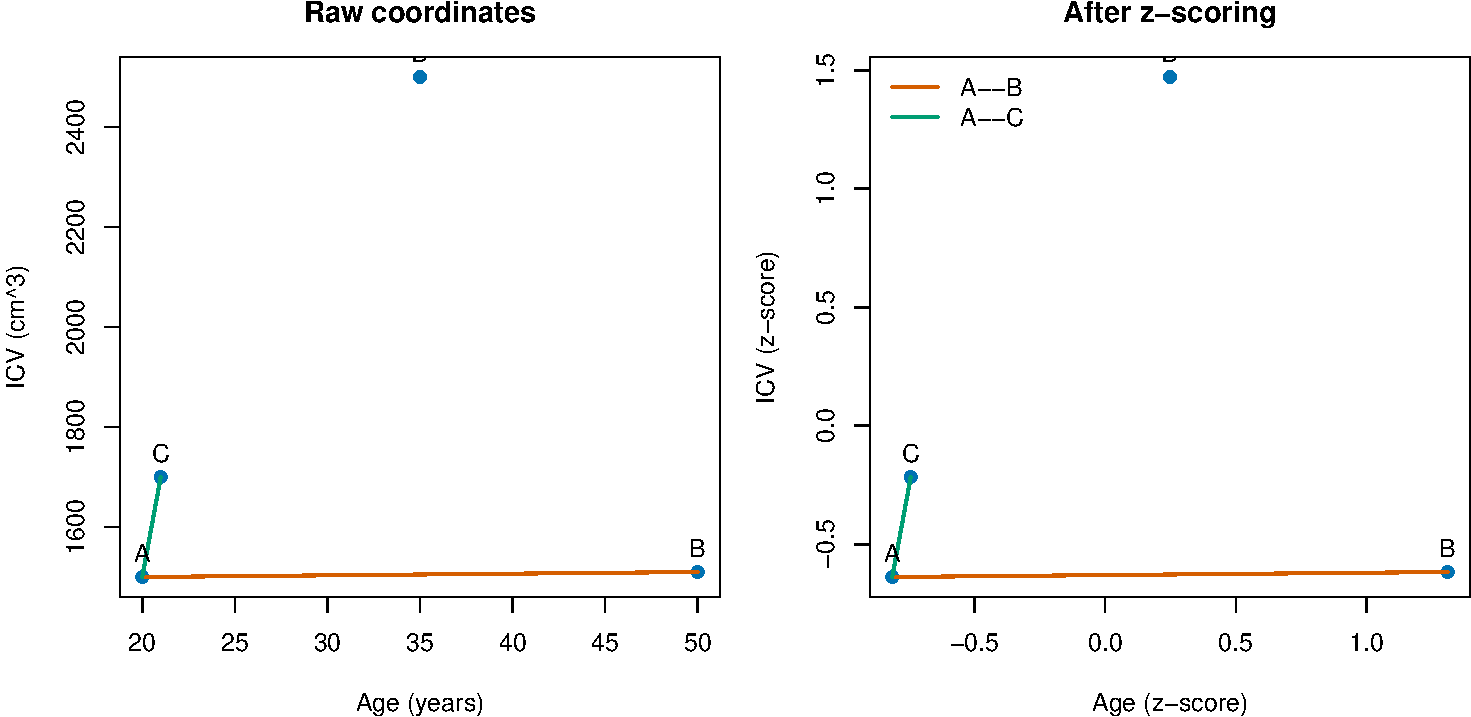
\includegraphics{11_mds_distances_files/figure-latex/two-dimensional-standardisation-1} 

}

\caption{The nearest profile to A changes after both variables are put on their standard-deviation scale. Segments compare A--B (orange) and A--C (green).}\label{fig:two-dimensional-standardisation}
\end{figure}

\begin{Shaded}
\begin{Highlighting}[]
\FunctionTok{par}\NormalTok{(old\_par)}
\end{Highlighting}
\end{Shaded}

\begin{Shaded}
\begin{Highlighting}[]
\NormalTok{brain }\OtherTok{\textless{}{-}} \FunctionTok{read\_csv}\NormalTok{(}\StringTok{"data/hippocampus\_memory\_age\_continuous.csv"}\NormalTok{, }\AttributeTok{show\_col\_types =} \ConstantTok{FALSE}\NormalTok{)}
\NormalTok{brain\_profile }\OtherTok{\textless{}{-}}\NormalTok{ brain }\SpecialCharTok{|\textgreater{}} \FunctionTok{select}\NormalTok{(memory\_score, hippocampal\_volume, age, ICV,}
\NormalTok{                                 motion, sleep\_hours, stress\_score)}

\NormalTok{d\_brain\_raw }\OtherTok{\textless{}{-}} \FunctionTok{dist}\NormalTok{(brain\_profile)}
\NormalTok{d\_brain\_z }\OtherTok{\textless{}{-}} \FunctionTok{dist}\NormalTok{(}\FunctionTok{scale}\NormalTok{(brain\_profile))}

\CommentTok{\# Mean squared pairwise difference identifies which variables drive raw distance.}
\NormalTok{raw\_contribution }\OtherTok{\textless{}{-}} \FunctionTok{sapply}\NormalTok{(brain\_profile, }\ControlFlowTok{function}\NormalTok{(v) }\FunctionTok{mean}\NormalTok{(}\FunctionTok{outer}\NormalTok{(v, v, }\StringTok{"{-}"}\NormalTok{)}\SpecialCharTok{\^{}}\DecValTok{2}\NormalTok{))}
\NormalTok{contribution }\OtherTok{\textless{}{-}} \FunctionTok{tibble}\NormalTok{(}\AttributeTok{variable =} \FunctionTok{names}\NormalTok{(raw\_contribution), }\AttributeTok{mean\_squared\_difference =}\NormalTok{ raw\_contribution)}
\NormalTok{knitr}\SpecialCharTok{::}\FunctionTok{kable}\NormalTok{(}\FunctionTok{arrange}\NormalTok{(contribution, }\FunctionTok{desc}\NormalTok{(mean\_squared\_difference)), }\AttributeTok{digits =} \DecValTok{2}\NormalTok{,}
             \AttributeTok{caption =} \StringTok{"Raw Euclidean distance is dominated by variables with large numerical scales."}\NormalTok{)}
\end{Highlighting}
\end{Shaded}

\begin{longtable}[]{@{}lr@{}}
\caption{Raw Euclidean distance is dominated by variables with large
numerical scales.}\tabularnewline
\toprule\noalign{}
variable & mean\_squared\_difference \\
\midrule\noalign{}
\endfirsthead
\toprule\noalign{}
variable & mean\_squared\_difference \\
\midrule\noalign{}
\endhead
\bottomrule\noalign{}
\endlastfoot
ICV & 21092.30 \\
age & 596.82 \\
memory\_score & 537.04 \\
stress\_score & 237.14 \\
sleep\_hours & 1.79 \\
hippocampal\_volume & 0.97 \\
motion & 0.01 \\
\end{longtable}

\begin{Shaded}
\begin{Highlighting}[]
\NormalTok{comparison\_brain }\OtherTok{\textless{}{-}} \FunctionTok{tibble}\NormalTok{(}\AttributeTok{raw =} \FunctionTok{as.vector}\NormalTok{(d\_brain\_raw), }\AttributeTok{z\_scored =} \FunctionTok{as.vector}\NormalTok{(d\_brain\_z))}
\FunctionTok{ggplot}\NormalTok{(comparison\_brain, }\FunctionTok{aes}\NormalTok{(raw, z\_scored)) }\SpecialCharTok{+}
  \FunctionTok{geom\_point}\NormalTok{(}\AttributeTok{colour =}\NormalTok{ blue, }\AttributeTok{alpha =} \FloatTok{.55}\NormalTok{) }\SpecialCharTok{+}
  \FunctionTok{geom\_smooth}\NormalTok{(}\AttributeTok{method =} \StringTok{"loess"}\NormalTok{, }\AttributeTok{se =} \ConstantTok{FALSE}\NormalTok{, }\AttributeTok{colour =}\NormalTok{ orange, }\AttributeTok{linewidth =} \DecValTok{1}\NormalTok{) }\SpecialCharTok{+}
  \FunctionTok{labs}\NormalTok{(}\AttributeTok{title =} \StringTok{"Raw and z{-}scored Euclidean distance answer different questions"}\NormalTok{,}
       \AttributeTok{x =} \StringTok{"Raw Euclidean distance"}\NormalTok{, }\AttributeTok{y =} \StringTok{"Euclidean distance after z{-}scoring"}\NormalTok{)}
\end{Highlighting}
\end{Shaded}

\begin{figure}

{\centering 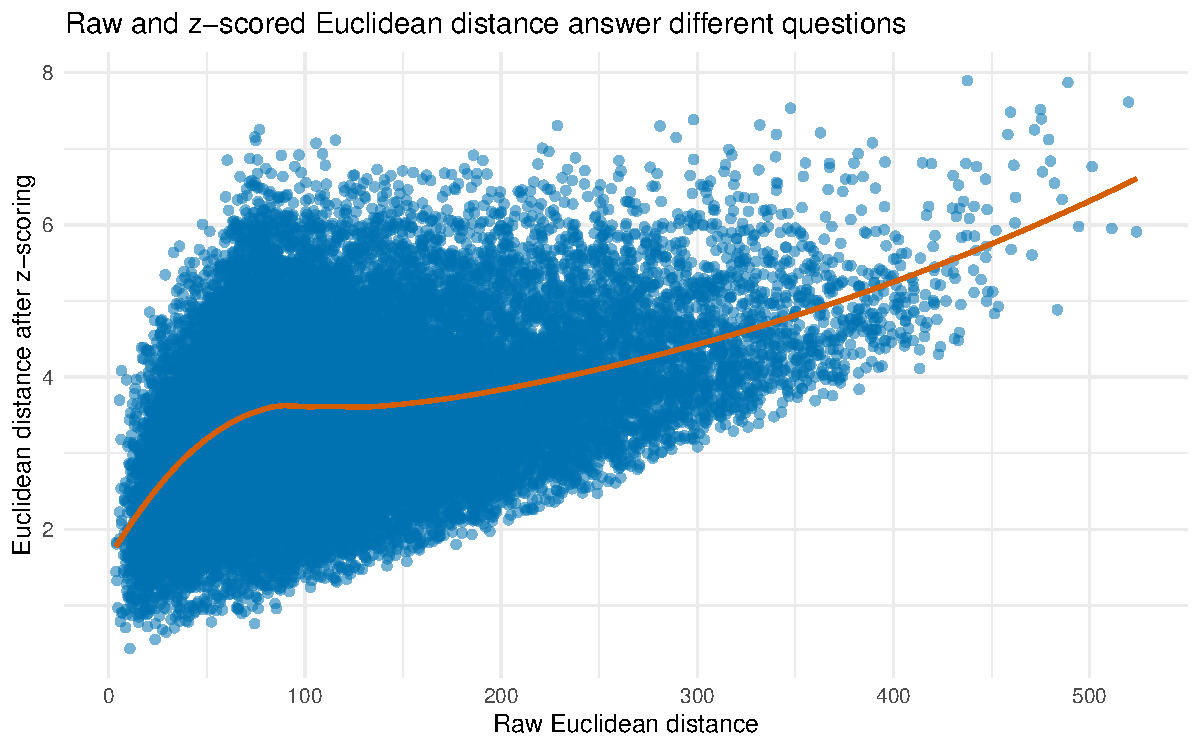
\includegraphics{11_mds_distances_files/figure-latex/euclidean-standardisation-plot-1} 

}

\caption{The two distances do not merely differ by a constant multiplier: standardisation can change which pairs of profiles are judged closest.}\label{fig:euclidean-standardisation-plot}
\end{figure}

\section{Worked example: Dutch dune-meadow
communities}\label{worked-example-dutch-dune-meadow-communities}

We use the real \texttt{dune} data distributed with the R package
\texttt{vegan}. It contains cover-class values for 30 plant species
recorded at 20 Dutch dune-meadow sites. The companion metadata record
soil A1-horizon thickness, moisture, management, land use and manure
level. The observations come from the dune-meadow study reported by
Jongman, ter Braak and van Tongeren (1987).

The course folder includes two redistributable CSV files extracted from
that dataset: \texttt{ecological\_communities.csv} contains the
species-by-site table and \texttt{ecological\_communities\_metadata.csv}
contains the site metadata. Species names are abbreviated as in the
original teaching dataset. The cover classes are ordered abundance
scores, not direct counts from equal-area sampling.

\begin{Shaded}
\begin{Highlighting}[]
\NormalTok{community }\OtherTok{\textless{}{-}} \FunctionTok{read\_csv}\NormalTok{(}\StringTok{"data/ecological\_communities.csv"}\NormalTok{, }\AttributeTok{show\_col\_types =} \ConstantTok{FALSE}\NormalTok{)}
\NormalTok{site\_metadata }\OtherTok{\textless{}{-}} \FunctionTok{read\_csv}\NormalTok{(}\StringTok{"data/ecological\_communities\_metadata.csv"}\NormalTok{, }\AttributeTok{show\_col\_types =} \ConstantTok{FALSE}\NormalTok{)}
\NormalTok{abundance }\OtherTok{\textless{}{-}}\NormalTok{ community }\SpecialCharTok{|\textgreater{}} \FunctionTok{select}\NormalTok{(}\SpecialCharTok{{-}}\NormalTok{site) }\SpecialCharTok{|\textgreater{}} \FunctionTok{as.data.frame}\NormalTok{()}
\FunctionTok{rownames}\NormalTok{(abundance) }\OtherTok{\textless{}{-}}\NormalTok{ community}\SpecialCharTok{$}\NormalTok{site}
\NormalTok{knitr}\SpecialCharTok{::}\FunctionTok{kable}\NormalTok{(}\FunctionTok{head}\NormalTok{(site\_metadata), }\AttributeTok{caption =} \StringTok{"First six rows of the site metadata. Full data are available in the CSV file."}\NormalTok{)}
\end{Highlighting}
\end{Shaded}

\begin{longtable}[]{@{}lrrllr@{}}
\caption{First six rows of the site metadata. Full data are available in
the CSV file.}\tabularnewline
\toprule\noalign{}
site & A1 & Moisture & Management & Use & Manure \\
\midrule\noalign{}
\endfirsthead
\toprule\noalign{}
site & A1 & Moisture & Management & Use & Manure \\
\midrule\noalign{}
\endhead
\bottomrule\noalign{}
\endlastfoot
site01 & 2.8 & 1 & SF & Haypastu & 4 \\
site02 & 3.5 & 1 & BF & Haypastu & 2 \\
site03 & 4.3 & 2 & SF & Haypastu & 4 \\
site04 & 4.2 & 2 & SF & Haypastu & 4 \\
site05 & 6.3 & 1 & HF & Hayfield & 2 \\
site06 & 4.3 & 1 & HF & Haypastu & 2 \\
\end{longtable}

\subsection{A first description of the community
data}\label{a-first-description-of-the-community-data}

Each row is one meadow site and each of the 30 species columns is an
ordinal cover-class score. Before computing any distances, ask how dense
the site profiles are and whether the sites differ in their recorded
management. The site total is a simple sum of cover scores, whereas
species richness is the number of species with a non-zero score. Neither
is a direct ecological abundance estimate, but both make the scale and
sparsity of the input tangible.

\begin{Shaded}
\begin{Highlighting}[]
\NormalTok{site\_description }\OtherTok{\textless{}{-}} \FunctionTok{tibble}\NormalTok{(}
  \AttributeTok{summary =} \FunctionTok{c}\NormalTok{(}\StringTok{"Number of sites"}\NormalTok{, }\StringTok{"Number of species"}\NormalTok{, }\StringTok{"Site{-}total cover score: min / median / max"}\NormalTok{,}
              \StringTok{"Species richness: min / median / max"}\NormalTok{),}
  \AttributeTok{value =} \FunctionTok{c}\NormalTok{(}
    \FunctionTok{nrow}\NormalTok{(abundance), }\FunctionTok{ncol}\NormalTok{(abundance),}
    \FunctionTok{sprintf}\NormalTok{(}\StringTok{"\%s / \%.1f / \%s"}\NormalTok{, }\FunctionTok{min}\NormalTok{(}\FunctionTok{rowSums}\NormalTok{(abundance)), }\FunctionTok{median}\NormalTok{(}\FunctionTok{rowSums}\NormalTok{(abundance)), }\FunctionTok{max}\NormalTok{(}\FunctionTok{rowSums}\NormalTok{(abundance))),}
    \FunctionTok{sprintf}\NormalTok{(}\StringTok{"\%s / \%.1f / \%s"}\NormalTok{, }\FunctionTok{min}\NormalTok{(}\FunctionTok{rowSums}\NormalTok{(abundance }\SpecialCharTok{\textgreater{}} \DecValTok{0}\NormalTok{)), }\FunctionTok{median}\NormalTok{(}\FunctionTok{rowSums}\NormalTok{(abundance }\SpecialCharTok{\textgreater{}} \DecValTok{0}\NormalTok{)), }\FunctionTok{max}\NormalTok{(}\FunctionTok{rowSums}\NormalTok{(abundance }\SpecialCharTok{\textgreater{}} \DecValTok{0}\NormalTok{)))}
\NormalTok{  )}
\NormalTok{)}
\NormalTok{knitr}\SpecialCharTok{::}\FunctionTok{kable}\NormalTok{(site\_description, }\AttributeTok{caption =} \StringTok{"Basic descriptive summary of the dune{-}meadow community matrix."}\NormalTok{)}
\end{Highlighting}
\end{Shaded}

\begin{longtable}[]{@{}ll@{}}
\caption{Basic descriptive summary of the dune-meadow community
matrix.}\tabularnewline
\toprule\noalign{}
summary & value \\
\midrule\noalign{}
\endfirsthead
\toprule\noalign{}
summary & value \\
\midrule\noalign{}
\endhead
\bottomrule\noalign{}
\endlastfoot
Number of sites & 20 \\
Number of species & 30 \\
Site-total cover score: min / median / max & 15 / 34.0 / 48 \\
Species richness: min / median / max & 5 / 9.5 / 14 \\
\end{longtable}

\begin{Shaded}
\begin{Highlighting}[]
\NormalTok{site\_profiles }\OtherTok{\textless{}{-}} \FunctionTok{tibble}\NormalTok{(}
  \AttributeTok{site =} \FunctionTok{rownames}\NormalTok{(abundance),}
  \AttributeTok{total\_cover\_score =} \FunctionTok{rowSums}\NormalTok{(abundance),}
  \AttributeTok{species\_richness =} \FunctionTok{rowSums}\NormalTok{(abundance }\SpecialCharTok{\textgreater{}} \DecValTok{0}\NormalTok{)}
\NormalTok{) }\SpecialCharTok{|\textgreater{}} \FunctionTok{left\_join}\NormalTok{(site\_metadata }\SpecialCharTok{|\textgreater{}} \FunctionTok{select}\NormalTok{(site, Management), }\AttributeTok{by =} \StringTok{"site"}\NormalTok{)}
\NormalTok{knitr}\SpecialCharTok{::}\FunctionTok{kable}\NormalTok{(}\FunctionTok{count}\NormalTok{(site\_profiles, Management, }\AttributeTok{name =} \StringTok{"sites"}\NormalTok{), }\AttributeTok{caption =} \StringTok{"Sites by recorded management category."}\NormalTok{)}
\end{Highlighting}
\end{Shaded}

\begin{longtable}[]{@{}lr@{}}
\caption{Sites by recorded management category.}\tabularnewline
\toprule\noalign{}
Management & sites \\
\midrule\noalign{}
\endfirsthead
\toprule\noalign{}
Management & sites \\
\midrule\noalign{}
\endhead
\bottomrule\noalign{}
\endlastfoot
BF & 3 \\
HF & 5 \\
NM & 6 \\
SF & 6 \\
\end{longtable}

\begin{Shaded}
\begin{Highlighting}[]
\FunctionTok{ggplot}\NormalTok{(site\_profiles, }\FunctionTok{aes}\NormalTok{(total\_cover\_score, species\_richness, }\AttributeTok{colour =}\NormalTok{ Management, }\AttributeTok{label =}\NormalTok{ site)) }\SpecialCharTok{+}
  \FunctionTok{geom\_point}\NormalTok{(}\AttributeTok{size =} \DecValTok{3}\NormalTok{) }\SpecialCharTok{+}
  \FunctionTok{geom\_text}\NormalTok{(}\AttributeTok{nudge\_y =} \FloatTok{.35}\NormalTok{, }\AttributeTok{show.legend =} \ConstantTok{FALSE}\NormalTok{) }\SpecialCharTok{+}
  \FunctionTok{labs}\NormalTok{(}\AttributeTok{title =} \StringTok{"Density and richness of the 20 site profiles"}\NormalTok{,}
       \AttributeTok{x =} \StringTok{"Sum of cover{-}class scores"}\NormalTok{, }\AttributeTok{y =} \StringTok{"Number of species present"}\NormalTok{)}
\end{Highlighting}
\end{Shaded}

\begin{figure}

{\centering 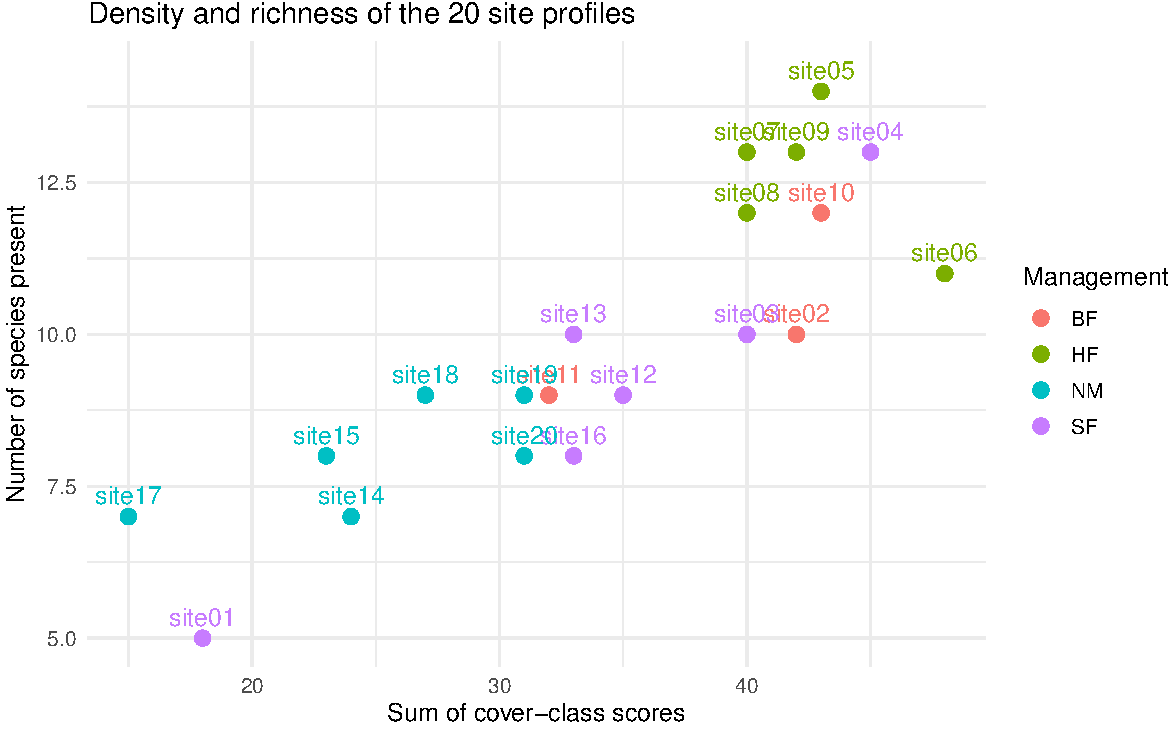
\includegraphics{11_mds_distances_files/figure-latex/community-description-plot-1} 

}

\caption{The sites differ both in total cover score and in the number of recorded species; these features are part of what a distance can respond to.}\label{fig:community-description-plot}
\end{figure}

\subsection{What does each distance
discriminate?}\label{what-does-each-distance-discriminate}

The relevant question is not whether numerical values of two distances
can be compared directly: they usually cannot. The question is whether a
distance separates sites in a way that corresponds to a defensible
notion of ecological difference.

Bray--Curtis compares the absolute difference in the species profiles
with the combined abundance of the two sites. Its denominator is
\(\sum_k(x_{ik}+x_{jk})\), twice the average total score of the pair.
Thus it creates a unitless \emph{relative} discrepancy and prevents a
uniformly larger abundance scale from mechanically creating arbitrarily
large distances. It does not make totals irrelevant: two sites with the
same composition but very different total abundance still have positive
Bray--Curtis dissimilarity.

For count-like observations, independent Poisson sampling is a useful
reminder: both the expected count and its variance grow with abundance.
Raw Euclidean distance therefore gives highly abundant species a large
role partly because they are numerically large and partly because their
sampling variation is larger. It is a pragmatic composition-oriented
dissimilarity. If total abundance is driven mainly by unequal sampling
effort, the effort problem should be addressed before interpreting any
distance.

\begin{Shaded}
\begin{Highlighting}[]
\NormalTok{bray\_curtis }\OtherTok{\textless{}{-}} \ControlFlowTok{function}\NormalTok{(x) \{}
\NormalTok{  x }\OtherTok{\textless{}{-}} \FunctionTok{as.matrix}\NormalTok{(x)}
\NormalTok{  n }\OtherTok{\textless{}{-}} \FunctionTok{nrow}\NormalTok{(x)}
\NormalTok{  out }\OtherTok{\textless{}{-}} \FunctionTok{matrix}\NormalTok{(}\DecValTok{0}\NormalTok{, n, n, }\AttributeTok{dimnames =} \FunctionTok{list}\NormalTok{(}\FunctionTok{rownames}\NormalTok{(x), }\FunctionTok{rownames}\NormalTok{(x)))}
  \ControlFlowTok{for}\NormalTok{ (i }\ControlFlowTok{in} \FunctionTok{seq\_len}\NormalTok{(n }\SpecialCharTok{{-}} \DecValTok{1}\NormalTok{)) \{}
    \ControlFlowTok{for}\NormalTok{ (j }\ControlFlowTok{in}\NormalTok{ (i }\SpecialCharTok{+} \DecValTok{1}\NormalTok{)}\SpecialCharTok{:}\NormalTok{n) \{}
\NormalTok{      out[i, j] }\OtherTok{\textless{}{-}}\NormalTok{ out[j, i] }\OtherTok{\textless{}{-}} \FunctionTok{sum}\NormalTok{(}\FunctionTok{abs}\NormalTok{(x[i, ] }\SpecialCharTok{{-}}\NormalTok{ x[j, ])) }\SpecialCharTok{/} \FunctionTok{sum}\NormalTok{(x[i, ] }\SpecialCharTok{+}\NormalTok{ x[j, ])}
\NormalTok{    \}}
\NormalTok{  \}}
  \FunctionTok{as.dist}\NormalTok{(out)}
\NormalTok{\}}

\NormalTok{d\_euclidean }\OtherTok{\textless{}{-}} \FunctionTok{dist}\NormalTok{(abundance, }\AttributeTok{method =} \StringTok{"euclidean"}\NormalTok{)}
\NormalTok{d\_bray }\OtherTok{\textless{}{-}} \FunctionTok{bray\_curtis}\NormalTok{(abundance)}

\NormalTok{relative\_abundance }\OtherTok{\textless{}{-}} \FunctionTok{sweep}\NormalTok{(}\FunctionTok{as.matrix}\NormalTok{(abundance), }\DecValTok{1}\NormalTok{, }\FunctionTok{rowSums}\NormalTok{(abundance), }\StringTok{"/"}\NormalTok{)}
\NormalTok{hellinger }\OtherTok{\textless{}{-}} \FunctionTok{sqrt}\NormalTok{(relative\_abundance)}
\NormalTok{d\_hellinger }\OtherTok{\textless{}{-}} \FunctionTok{dist}\NormalTok{(hellinger, }\AttributeTok{method =} \StringTok{"euclidean"}\NormalTok{)}
\end{Highlighting}
\end{Shaded}

\subsection{Hellinger transformation: composition in Euclidean
geometry}\label{hellinger-transformation-composition-in-euclidean-geometry}

For each site, Hellinger transformation first changes cover scores into
a composition (each row sums to one), then takes the square root of each
relative abundance. The resulting distance is

\[d_H(i,j)=\left[\sum_{k=1}^p\left(\sqrt{\frac{x_{ik}}{x_{i+}}}-
\sqrt{\frac{x_{jk}}{x_{j+}}}\right)^2\right]^{1/2}.\]

It therefore compares composition rather than raw total cover, while the
square root reduces the dominance of common species. Most importantly
for this unit, the transformed rows lie in an ordinary Euclidean space:
their Euclidean distances can be represented exactly by a sufficiently
high-dimensional MDS configuration. Hellinger transformation is not a
generic replacement for Bray--Curtis; it answers a closely related but
distinct question.

\begin{Shaded}
\begin{Highlighting}[]
\NormalTok{distance\_long }\OtherTok{\textless{}{-}} \FunctionTok{bind\_rows}\NormalTok{(}
  \FunctionTok{as.data.frame}\NormalTok{(}\FunctionTok{as.table}\NormalTok{(}\FunctionTok{as.matrix}\NormalTok{(d\_bray))) }\SpecialCharTok{|\textgreater{}} \FunctionTok{rename}\NormalTok{(}\AttributeTok{site\_1 =}\NormalTok{ Var1, }\AttributeTok{site\_2 =}\NormalTok{ Var2, }\AttributeTok{distance =}\NormalTok{ Freq) }\SpecialCharTok{|\textgreater{}} \FunctionTok{mutate}\NormalTok{(}\AttributeTok{metric =} \StringTok{"Bray{-}{-}Curtis"}\NormalTok{),}
  \FunctionTok{as.data.frame}\NormalTok{(}\FunctionTok{as.table}\NormalTok{(}\FunctionTok{as.matrix}\NormalTok{(d\_hellinger))) }\SpecialCharTok{|\textgreater{}} \FunctionTok{rename}\NormalTok{(}\AttributeTok{site\_1 =}\NormalTok{ Var1, }\AttributeTok{site\_2 =}\NormalTok{ Var2, }\AttributeTok{distance =}\NormalTok{ Freq) }\SpecialCharTok{|\textgreater{}} \FunctionTok{mutate}\NormalTok{(}\AttributeTok{metric =} \StringTok{"Euclidean after Hellinger"}\NormalTok{)}
\NormalTok{) }\SpecialCharTok{|\textgreater{}} \FunctionTok{filter}\NormalTok{(site\_1 }\SpecialCharTok{!=}\NormalTok{ site\_2)}

\FunctionTok{ggplot}\NormalTok{(distance\_long, }\FunctionTok{aes}\NormalTok{(site\_1, site\_2, }\AttributeTok{fill =}\NormalTok{ distance)) }\SpecialCharTok{+}
  \FunctionTok{geom\_tile}\NormalTok{(}\AttributeTok{colour =} \StringTok{"white"}\NormalTok{) }\SpecialCharTok{+}
  \FunctionTok{geom\_text}\NormalTok{(}\FunctionTok{aes}\NormalTok{(}\AttributeTok{label =} \FunctionTok{sprintf}\NormalTok{(}\StringTok{"\%.2f"}\NormalTok{, distance)), }\AttributeTok{size =} \DecValTok{3}\NormalTok{) }\SpecialCharTok{+}
  \FunctionTok{facet\_wrap}\NormalTok{(}\SpecialCharTok{\textasciitilde{}}\NormalTok{ metric) }\SpecialCharTok{+}
  \FunctionTok{scale\_fill\_viridis\_c}\NormalTok{(}\AttributeTok{option =} \StringTok{"C"}\NormalTok{) }\SpecialCharTok{+}
  \FunctionTok{coord\_fixed}\NormalTok{() }\SpecialCharTok{+}
  \FunctionTok{labs}\NormalTok{(}\AttributeTok{title =} \StringTok{"Pairwise distances depend on the question"}\NormalTok{, }\AttributeTok{x =} \ConstantTok{NULL}\NormalTok{, }\AttributeTok{y =} \ConstantTok{NULL}\NormalTok{, }\AttributeTok{fill =} \StringTok{"Distance"}\NormalTok{) }\SpecialCharTok{+}
  \FunctionTok{theme}\NormalTok{(}\AttributeTok{axis.text.x =} \FunctionTok{element\_text}\NormalTok{(}\AttributeTok{angle =} \DecValTok{45}\NormalTok{, }\AttributeTok{hjust =} \DecValTok{1}\NormalTok{))}
\end{Highlighting}
\end{Shaded}

\begin{figure}

{\centering 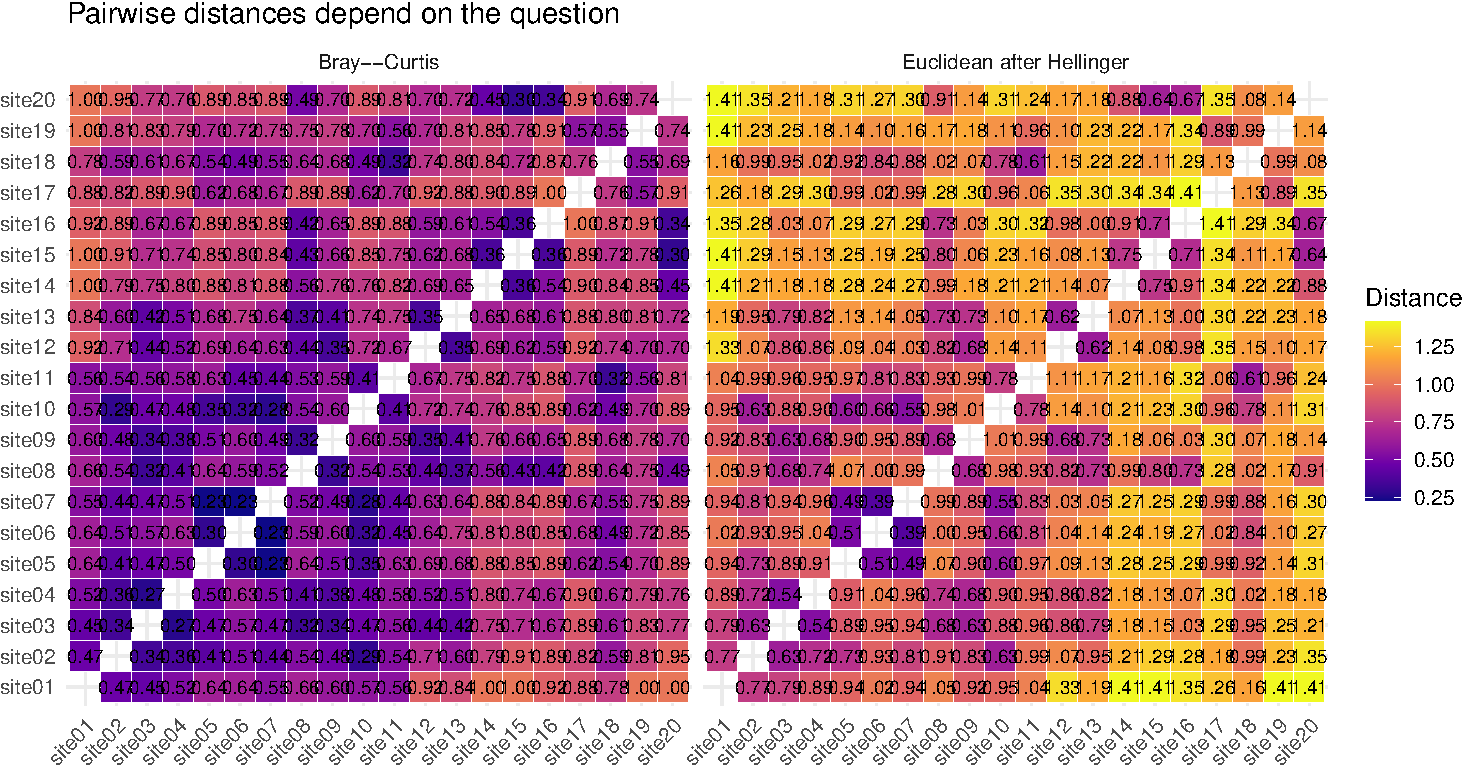
\includegraphics{11_mds_distances_files/figure-latex/compare-distance-heatmaps-1} 

}

\caption{Bray--Curtis and Euclidean distance after Hellinger standardisation encode different, but related, composition contrasts. The numerical values use different scales; compare the pattern of close and distant pairs instead.}\label{fig:compare-distance-heatmaps}
\end{figure}

\subsection{Bray--Curtis versus standardised Euclidean
distance}\label{braycurtis-versus-standardised-euclidean-distance}

Hellinger standardisation first converts each site profile to relative
abundance and then takes square roots. The square root reduces the
dominance of common species and makes Euclidean geometry available. It
is not the same as applying a column-wise z-score: z-scoring gives every
species equal variance across sites and can make a rare species
influential merely because it varies little.

\begin{Shaded}
\begin{Highlighting}[]
\NormalTok{comparison }\OtherTok{\textless{}{-}} \FunctionTok{tibble}\NormalTok{(}
  \AttributeTok{bray =} \FunctionTok{as.vector}\NormalTok{(d\_bray),}
  \AttributeTok{hellinger\_euclidean =} \FunctionTok{as.vector}\NormalTok{(d\_hellinger)}
\NormalTok{)}

\FunctionTok{ggplot}\NormalTok{(comparison, }\FunctionTok{aes}\NormalTok{(bray, hellinger\_euclidean)) }\SpecialCharTok{+}
  \FunctionTok{geom\_point}\NormalTok{(}\AttributeTok{size =} \FloatTok{2.4}\NormalTok{, }\AttributeTok{colour =}\NormalTok{ blue, }\AttributeTok{alpha =} \FloatTok{.8}\NormalTok{) }\SpecialCharTok{+}
  \FunctionTok{geom\_smooth}\NormalTok{(}\AttributeTok{method =} \StringTok{"loess"}\NormalTok{, }\AttributeTok{se =} \ConstantTok{FALSE}\NormalTok{, }\AttributeTok{colour =}\NormalTok{ orange, }\AttributeTok{linewidth =} \DecValTok{1}\NormalTok{) }\SpecialCharTok{+}
  \FunctionTok{labs}\NormalTok{(}
    \AttributeTok{title =} \StringTok{"Do the two distances discriminate similar site pairs?"}\NormalTok{,}
    \AttributeTok{subtitle =} \FunctionTok{paste}\NormalTok{(}\StringTok{"Spearman rank correlation ="}\NormalTok{, }\FunctionTok{round}\NormalTok{(}\FunctionTok{cor}\NormalTok{(comparison}\SpecialCharTok{$}\NormalTok{bray, comparison}\SpecialCharTok{$}\NormalTok{hellinger\_euclidean, }\AttributeTok{method =} \StringTok{"spearman"}\NormalTok{), }\DecValTok{2}\NormalTok{)),}
    \AttributeTok{x =} \StringTok{"Bray{-}{-}Curtis dissimilarity"}\NormalTok{,}
    \AttributeTok{y =} \StringTok{"Euclidean distance after Hellinger standardisation"}
\NormalTok{  )}
\end{Highlighting}
\end{Shaded}

\begin{figure}

{\centering 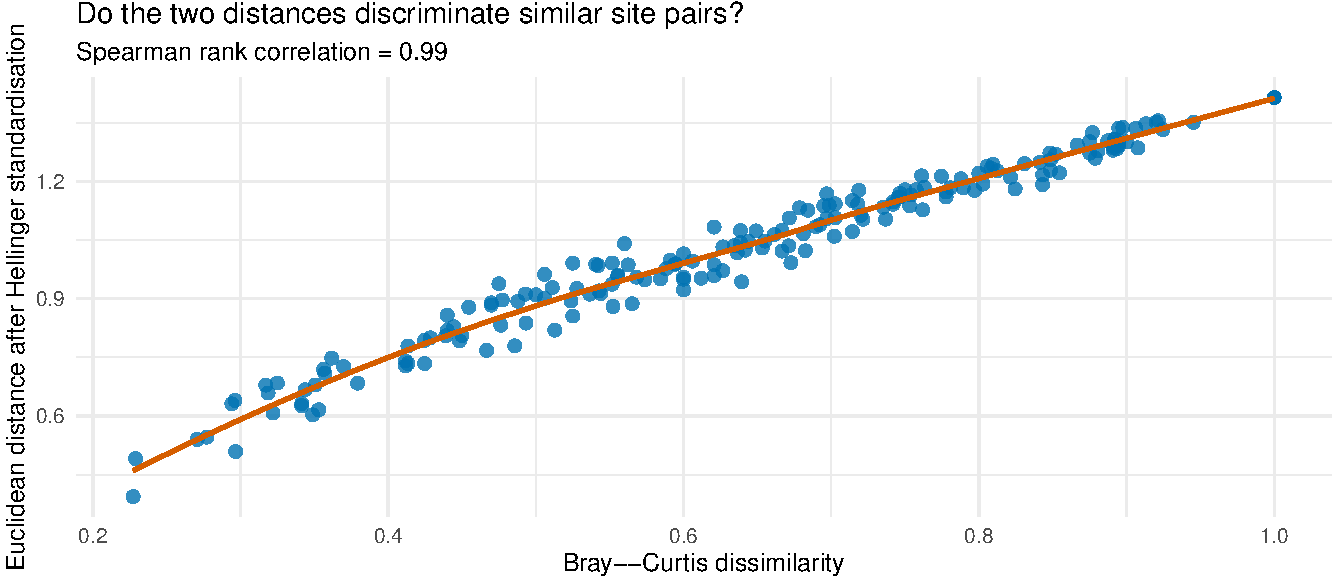
\includegraphics{11_mds_distances_files/figure-latex/bray-hellinger-agreement-1} 

}

\caption{The metrics need not have the same numerical scale. Their rank agreement tells us whether they broadly discriminate the same pairs of sites.}\label{fig:bray-hellinger-agreement}
\end{figure}

Neither distance is universally better.

{\def\LTcaptype{none} % do not increment counter
\begin{longtable}[]{@{}
  >{\raggedright\arraybackslash}p{(\linewidth - 4\tabcolsep) * \real{0.3333}}
  >{\raggedright\arraybackslash}p{(\linewidth - 4\tabcolsep) * \real{0.3333}}
  >{\raggedright\arraybackslash}p{(\linewidth - 4\tabcolsep) * \real{0.3333}}@{}}
\toprule\noalign{}
\begin{minipage}[b]{\linewidth}\raggedright
If the scientific emphasis is\ldots{}
\end{minipage} & \begin{minipage}[b]{\linewidth}\raggedright
Prefer\ldots{}
\end{minipage} & \begin{minipage}[b]{\linewidth}\raggedright
Why
\end{minipage} \\
\midrule\noalign{}
\endhead
\bottomrule\noalign{}
\endlastfoot
A traditional ecological comparison of abundance profiles, with shared
zeros ignored & Bray--Curtis & Its denominator gives a relative, bounded
discrepancy and it is widely interpretable for community composition. \\
A composition analysis requiring Euclidean geometry, PCA-like tools or
an exactly Euclidean MDS input & Hellinger transformation + Euclidean
distance & It compares transformed relative abundances and gives a
Euclidean distance matrix. \\
Equal influence for every species after accounting for each species'
variability & Column-standardised Euclidean distance & This is a
different question; use it only when equal species variance is
substantively intended. \\
\end{longtable}
}

Report the selected definition and show a sensitivity comparison when
conclusions depend on it. A result is reproducible only if the
transformations, distance and included species are documented.

\subsection{Scaling is also a modelling
choice}\label{scaling-is-also-a-modelling-choice}

Column-wise standardisation is valuable for generic multivariate
measurements in different units, but it is not a default repair for
species-abundance tables. To make the contrast visible, we compare
Hellinger Euclidean distance with Euclidean distance after species-wise
z-scoring.

\begin{Shaded}
\begin{Highlighting}[]
\NormalTok{scaled\_distance }\OtherTok{\textless{}{-}} \FunctionTok{as.matrix}\NormalTok{(}\FunctionTok{dist}\NormalTok{(}\FunctionTok{scale}\NormalTok{(abundance)))}
\NormalTok{hellinger\_distance }\OtherTok{\textless{}{-}} \FunctionTok{as.matrix}\NormalTok{(d\_hellinger)}

\FunctionTok{plot}\NormalTok{(hellinger\_distance[}\FunctionTok{upper.tri}\NormalTok{(hellinger\_distance)], scaled\_distance[}\FunctionTok{upper.tri}\NormalTok{(scaled\_distance)],}
     \AttributeTok{pch =} \DecValTok{19}\NormalTok{, }\AttributeTok{col =} \FunctionTok{adjustcolor}\NormalTok{(blue, }\FloatTok{.7}\NormalTok{),}
     \AttributeTok{xlab =} \StringTok{"Euclidean distance after Hellinger transformation"}\NormalTok{,}
     \AttributeTok{ylab =} \StringTok{"Euclidean distance after species{-}wise z{-}scoring"}\NormalTok{,}
     \AttributeTok{main =} \StringTok{"Different standardisations encode different questions"}\NormalTok{)}
\FunctionTok{abline}\NormalTok{(}\FunctionTok{lm}\NormalTok{(scaled\_distance[}\FunctionTok{upper.tri}\NormalTok{(scaled\_distance)] }\SpecialCharTok{\textasciitilde{}}\NormalTok{ hellinger\_distance[}\FunctionTok{upper.tri}\NormalTok{(hellinger\_distance)]),}
       \AttributeTok{col =}\NormalTok{ orange, }\AttributeTok{lwd =} \DecValTok{2}\NormalTok{)}
\end{Highlighting}
\end{Shaded}

\begin{figure}

{\centering 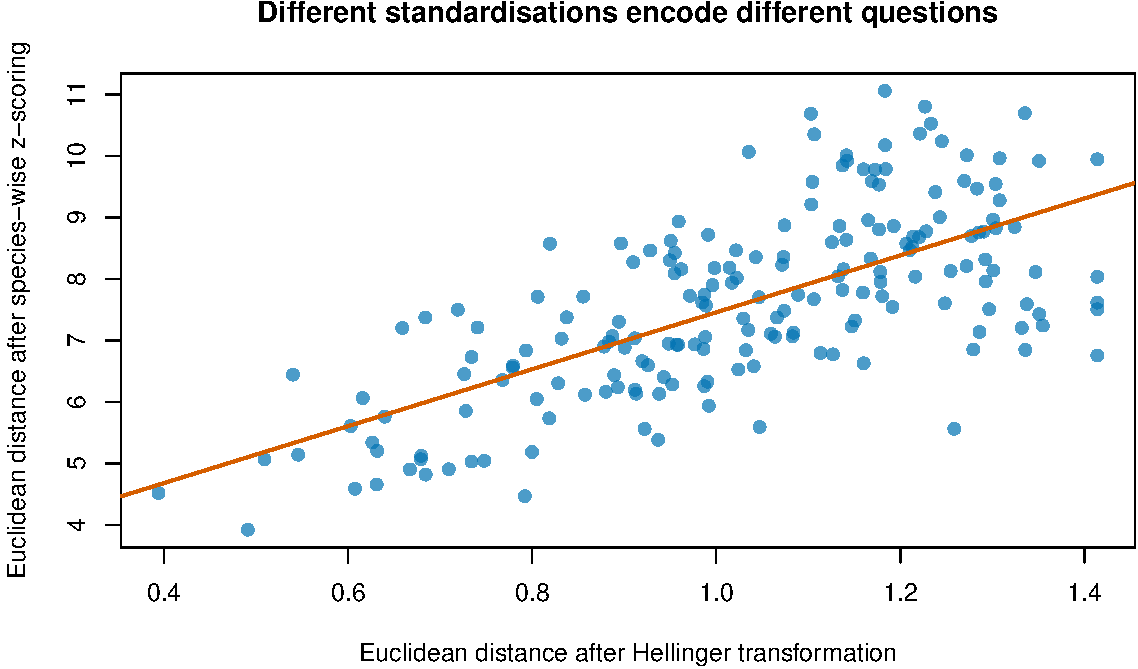
\includegraphics{11_mds_distances_files/figure-latex/scaling-example-1} 

}

\caption{Standardisation changes Euclidean distances by changing the relative influence of variables.}\label{fig:scaling-example}
\end{figure}

\section{Classical MDS: turn distances into
coordinates}\label{classical-mds-turn-distances-into-coordinates}

MDS receives a distance matrix and returns coordinates. Classical MDS
finds a Euclidean configuration whose interpoint distances reproduce the
input as closely as possible. The configuration can then be plotted just
like ordinary coordinates.

\subsection{Spectral decomposition, one matrix at a
time}\label{spectral-decomposition-one-matrix-at-a-time}

The construction is easiest to see with only three objects. Reuse the
three points introduced earlier: A = (0, 0), B = (3, 4), and C = (3, 0).
We know their geometry, so we can check whether MDS recovers it from
distances alone. The coordinates are used only to create the example;
every following step uses the distance matrix.

\subsubsection{Step 1 --- distances and squared
distances}\label{step-1-distances-and-squared-distances}

Let \(D\) contain the pairwise distances and let \(D^{(2)}\) contain
their squares:

\[D=(d_{ij}), \qquad D^{(2)}=(d_{ij}^2).\]

\begin{Shaded}
\begin{Highlighting}[]
\NormalTok{X\_original }\OtherTok{\textless{}{-}} \FunctionTok{rbind}\NormalTok{(}\AttributeTok{A =} \FunctionTok{c}\NormalTok{(}\DecValTok{0}\NormalTok{, }\DecValTok{0}\NormalTok{), }\AttributeTok{B =} \FunctionTok{c}\NormalTok{(}\DecValTok{3}\NormalTok{, }\DecValTok{4}\NormalTok{), }\AttributeTok{C =} \FunctionTok{c}\NormalTok{(}\DecValTok{3}\NormalTok{, }\DecValTok{0}\NormalTok{))}
\NormalTok{d\_orig }\OtherTok{\textless{}{-}} \FunctionTok{tibble}\NormalTok{(}\AttributeTok{object =} \FunctionTok{rownames}\NormalTok{(X\_original), }\AttributeTok{x =}\NormalTok{ X\_original[, }\DecValTok{1}\NormalTok{], }\AttributeTok{y =}\NormalTok{ X\_original[, }\DecValTok{2}\NormalTok{])}
\NormalTok{D }\OtherTok{\textless{}{-}} \FunctionTok{as.matrix}\NormalTok{(}\FunctionTok{dist}\NormalTok{(X\_original))}
\NormalTok{D2 }\OtherTok{\textless{}{-}}\NormalTok{ D}\SpecialCharTok{\^{}}\DecValTok{2}

\NormalTok{knitr}\SpecialCharTok{::}\FunctionTok{kable}\NormalTok{(d\_orig, }\AttributeTok{digits =} \DecValTok{2}\NormalTok{, }\AttributeTok{caption =} \StringTok{"Original two{-}dimensional coordinates used only to create this small example."}\NormalTok{)}
\end{Highlighting}
\end{Shaded}

\begin{longtable}[]{@{}lrr@{}}
\caption{Original two-dimensional coordinates used only to create this
small example.}\tabularnewline
\toprule\noalign{}
object & x & y \\
\midrule\noalign{}
\endfirsthead
\toprule\noalign{}
object & x & y \\
\midrule\noalign{}
\endhead
\bottomrule\noalign{}
\endlastfoot
A & 0 & 0 \\
B & 3 & 4 \\
C & 3 & 0 \\
\end{longtable}

\begin{Shaded}
\begin{Highlighting}[]
\NormalTok{knitr}\SpecialCharTok{::}\FunctionTok{kable}\NormalTok{(D, }\AttributeTok{digits =} \DecValTok{2}\NormalTok{, }\AttributeTok{caption =} \StringTok{"Step 1a: distance matrix D."}\NormalTok{)}
\end{Highlighting}
\end{Shaded}

\begin{longtable}[]{@{}lrrr@{}}
\caption{Step 1a: distance matrix D.}\tabularnewline
\toprule\noalign{}
& A & B & C \\
\midrule\noalign{}
\endfirsthead
\toprule\noalign{}
& A & B & C \\
\midrule\noalign{}
\endhead
\bottomrule\noalign{}
\endlastfoot
A & 0 & 5 & 3 \\
B & 5 & 0 & 4 \\
C & 3 & 4 & 0 \\
\end{longtable}

\begin{Shaded}
\begin{Highlighting}[]
\NormalTok{knitr}\SpecialCharTok{::}\FunctionTok{kable}\NormalTok{(D2, }\AttributeTok{digits =} \DecValTok{2}\NormalTok{, }\AttributeTok{caption =} \StringTok{"Step 1b: squared{-}distance matrix D\^{}(2)."}\NormalTok{)}
\end{Highlighting}
\end{Shaded}

\begin{longtable}[]{@{}lrrr@{}}
\caption{Step 1b: squared-distance matrix D\^{}(2).}\tabularnewline
\toprule\noalign{}
& A & B & C \\
\midrule\noalign{}
\endfirsthead
\toprule\noalign{}
& A & B & C \\
\midrule\noalign{}
\endhead
\bottomrule\noalign{}
\endlastfoot
A & 0 & 25 & 9 \\
B & 25 & 0 & 16 \\
C & 9 & 16 & 0 \\
\end{longtable}

\begin{Shaded}
\begin{Highlighting}[]
\FunctionTok{plot}\NormalTok{(d\_orig}\SpecialCharTok{$}\NormalTok{x, d\_orig}\SpecialCharTok{$}\NormalTok{y, }\AttributeTok{asp =} \DecValTok{1}\NormalTok{, }\AttributeTok{pch =} \DecValTok{19}\NormalTok{, }\AttributeTok{col =}\NormalTok{ blue, }\AttributeTok{xlab =} \StringTok{"Original coordinate 1"}\NormalTok{,}
     \AttributeTok{ylab =} \StringTok{"Original coordinate 2"}\NormalTok{, }\AttributeTok{main =} \StringTok{"Original data: d\_orig"}\NormalTok{,}
     \AttributeTok{xlim =} \FunctionTok{c}\NormalTok{(}\SpecialCharTok{{-}}\DecValTok{1}\NormalTok{, }\DecValTok{4}\NormalTok{), }\AttributeTok{ylim =} \FunctionTok{c}\NormalTok{(}\SpecialCharTok{{-}}\DecValTok{1}\NormalTok{, }\DecValTok{5}\NormalTok{))}
\FunctionTok{text}\NormalTok{(d\_orig}\SpecialCharTok{$}\NormalTok{x, d\_orig}\SpecialCharTok{$}\NormalTok{y, }\AttributeTok{labels =}\NormalTok{ d\_orig}\SpecialCharTok{$}\NormalTok{object, }\AttributeTok{pos =} \DecValTok{3}\NormalTok{)}
\end{Highlighting}
\end{Shaded}

\begin{center}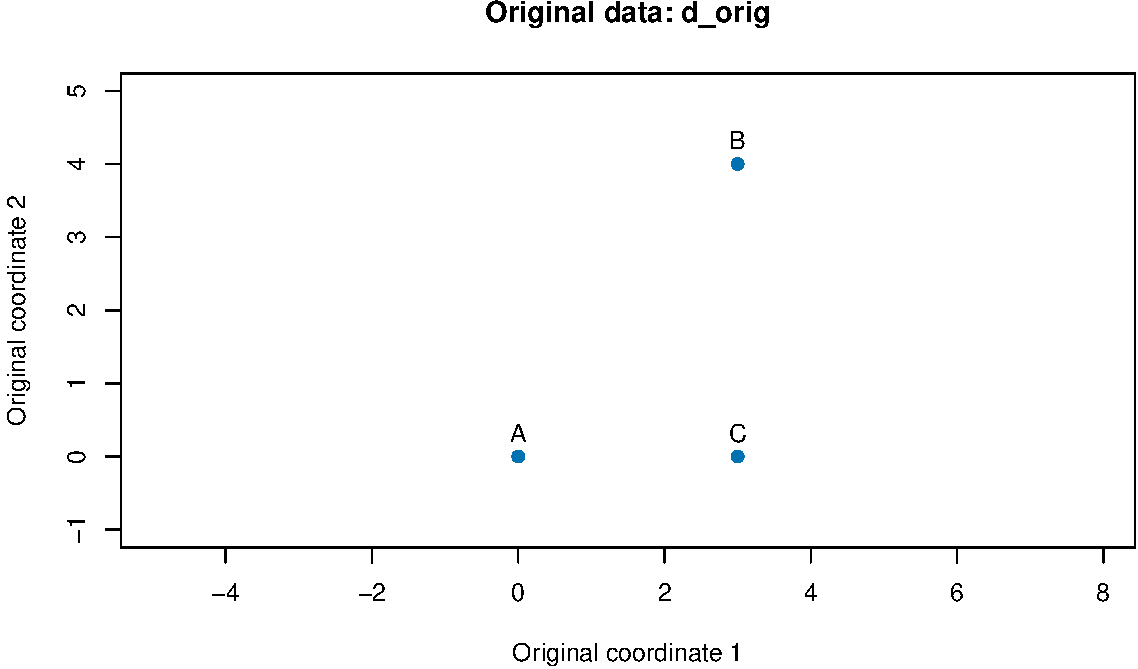
\includegraphics{11_mds_distances_files/figure-latex/spectral-step-1-1} \end{center}

\subsubsection{Step 2 --- centre the squared
distances}\label{step-2-centre-the-squared-distances}

With \(n=3\), the centring matrix is

\[J=I_n-\frac{1}{n}\mathbf{1}\mathbf{1}^T.\]

Double-centring converts squared distances into a Gram matrix:

\[B=-\frac{1}{2}JD^{(2)}J.\]

For exactly Euclidean distances, \(B\) is the centred inner-product
matrix \(X_cX_c^T\), where \(X_c\) denotes centred coordinates. It is
symmetric and positive semidefinite.

\begin{Shaded}
\begin{Highlighting}[]
\NormalTok{n }\OtherTok{\textless{}{-}} \FunctionTok{nrow}\NormalTok{(D)}
\NormalTok{J }\OtherTok{\textless{}{-}} \FunctionTok{diag}\NormalTok{(n) }\SpecialCharTok{{-}} \FunctionTok{matrix}\NormalTok{(}\DecValTok{1} \SpecialCharTok{/}\NormalTok{ n, n, n)}
\NormalTok{B }\OtherTok{\textless{}{-}} \SpecialCharTok{{-}}\FloatTok{0.5} \SpecialCharTok{*}\NormalTok{ J }\SpecialCharTok{\%*\%}\NormalTok{ D2 }\SpecialCharTok{\%*\%}\NormalTok{ J}

\NormalTok{knitr}\SpecialCharTok{::}\FunctionTok{kable}\NormalTok{(J, }\AttributeTok{digits =} \DecValTok{3}\NormalTok{, }\AttributeTok{caption =} \StringTok{"Step 2a: centring matrix J."}\NormalTok{)}
\end{Highlighting}
\end{Shaded}

\begin{longtable}[]{@{}rrr@{}}
\caption{Step 2a: centring matrix J.}\tabularnewline
\toprule\noalign{}
\endfirsthead
\endhead
\bottomrule\noalign{}
\endlastfoot
0.667 & -0.333 & -0.333 \\
-0.333 & 0.667 & -0.333 \\
-0.333 & -0.333 & 0.667 \\
\end{longtable}

\begin{Shaded}
\begin{Highlighting}[]
\NormalTok{knitr}\SpecialCharTok{::}\FunctionTok{kable}\NormalTok{(B, }\AttributeTok{digits =} \DecValTok{3}\NormalTok{, }\AttributeTok{caption =} \StringTok{"Step 2b: centred Gram matrix B."}\NormalTok{)}
\end{Highlighting}
\end{Shaded}

\begin{longtable}[]{@{}rrr@{}}
\caption{Step 2b: centred Gram matrix B.}\tabularnewline
\toprule\noalign{}
\endfirsthead
\endhead
\bottomrule\noalign{}
\endlastfoot
5.778 & -5.556 & -0.222 \\
-5.556 & 8.111 & -2.556 \\
-0.222 & -2.556 & 2.778 \\
\end{longtable}

\subsubsection{Step 3 --- spectral decomposition of
B}\label{step-3-spectral-decomposition-of-b}

Because \(B\) is real and symmetric, the spectral theorem gives

\[B=Q\Lambda Q^T,\]

where the columns of \(Q\) are orthonormal eigenvectors and \(\Lambda\)
is a diagonal matrix of eigenvalues. The number of positive eigenvalues
is the dimension needed for an exact Euclidean representation (apart
from numerical rounding).

\begin{Shaded}
\begin{Highlighting}[]
\NormalTok{decomposition }\OtherTok{\textless{}{-}} \FunctionTok{eigen}\NormalTok{(B, }\AttributeTok{symmetric =} \ConstantTok{TRUE}\NormalTok{)}
\NormalTok{Q }\OtherTok{\textless{}{-}}\NormalTok{ decomposition}\SpecialCharTok{$}\NormalTok{vectors}
\NormalTok{Lambda }\OtherTok{\textless{}{-}} \FunctionTok{diag}\NormalTok{(decomposition}\SpecialCharTok{$}\NormalTok{values)}
\FunctionTok{rownames}\NormalTok{(Q) }\OtherTok{\textless{}{-}} \FunctionTok{rownames}\NormalTok{(D)}
\FunctionTok{rownames}\NormalTok{(Lambda) }\OtherTok{\textless{}{-}} \FunctionTok{colnames}\NormalTok{(Lambda) }\OtherTok{\textless{}{-}} \FunctionTok{paste0}\NormalTok{(}\StringTok{"lambda"}\NormalTok{, }\FunctionTok{seq\_len}\NormalTok{(n))}
\FunctionTok{colnames}\NormalTok{(Q) }\OtherTok{\textless{}{-}} \FunctionTok{paste0}\NormalTok{(}\StringTok{"q"}\NormalTok{, }\FunctionTok{seq\_len}\NormalTok{(n))}

\NormalTok{knitr}\SpecialCharTok{::}\FunctionTok{kable}\NormalTok{(Q, }\AttributeTok{digits =} \DecValTok{3}\NormalTok{, }\AttributeTok{caption =} \StringTok{"Step 3a: eigenvector matrix Q."}\NormalTok{)}
\end{Highlighting}
\end{Shaded}

\begin{longtable}[]{@{}lrrr@{}}
\caption{Step 3a: eigenvector matrix Q.}\tabularnewline
\toprule\noalign{}
& q1 & q2 & q3 \\
\midrule\noalign{}
\endfirsthead
\toprule\noalign{}
& q1 & q2 & q3 \\
\midrule\noalign{}
\endhead
\bottomrule\noalign{}
\endlastfoot
A & 0.598 & -0.556 & 0.577 \\
B & -0.781 & -0.240 & 0.577 \\
C & 0.183 & 0.796 & 0.577 \\
\end{longtable}

\begin{Shaded}
\begin{Highlighting}[]
\NormalTok{knitr}\SpecialCharTok{::}\FunctionTok{kable}\NormalTok{(Lambda, }\AttributeTok{digits =} \DecValTok{3}\NormalTok{, }\AttributeTok{caption =} \StringTok{"Step 3b: diagonal eigenvalue matrix Lambda."}\NormalTok{)}
\end{Highlighting}
\end{Shaded}

\begin{longtable}[]{@{}lrrr@{}}
\caption{Step 3b: diagonal eigenvalue matrix Lambda.}\tabularnewline
\toprule\noalign{}
& lambda1 & lambda2 & lambda3 \\
\midrule\noalign{}
\endfirsthead
\toprule\noalign{}
& lambda1 & lambda2 & lambda3 \\
\midrule\noalign{}
\endhead
\bottomrule\noalign{}
\endlastfoot
lambda1 & 12.964 & 0.000 & 0 \\
lambda2 & 0.000 & 3.703 & 0 \\
lambda3 & 0.000 & 0.000 & 0 \\
\end{longtable}

\begin{Shaded}
\begin{Highlighting}[]
\NormalTok{knitr}\SpecialCharTok{::}\FunctionTok{kable}\NormalTok{(}\FunctionTok{tibble}\NormalTok{(}\AttributeTok{dimension =} \FunctionTok{seq\_len}\NormalTok{(n), }\AttributeTok{eigenvalue =}\NormalTok{ decomposition}\SpecialCharTok{$}\NormalTok{values),}
             \AttributeTok{digits =} \DecValTok{3}\NormalTok{, }\AttributeTok{caption =} \StringTok{"Step 3c: eigenvalues in descending order."}\NormalTok{)}
\end{Highlighting}
\end{Shaded}

\begin{longtable}[]{@{}rr@{}}
\caption{Step 3c: eigenvalues in descending order.}\tabularnewline
\toprule\noalign{}
dimension & eigenvalue \\
\midrule\noalign{}
\endfirsthead
\toprule\noalign{}
dimension & eigenvalue \\
\midrule\noalign{}
\endhead
\bottomrule\noalign{}
\endlastfoot
1 & 12.964 \\
2 & 3.703 \\
3 & 0.000 \\
\end{longtable}

\begin{Shaded}
\begin{Highlighting}[]
\NormalTok{q\_plot }\OtherTok{\textless{}{-}} \FunctionTok{tibble}\NormalTok{(}\AttributeTok{object =} \FunctionTok{rownames}\NormalTok{(Q), }\AttributeTok{q1 =}\NormalTok{ Q[, }\DecValTok{1}\NormalTok{], }\AttributeTok{q2 =}\NormalTok{ Q[, }\DecValTok{2}\NormalTok{])}
\FunctionTok{plot}\NormalTok{(q\_plot}\SpecialCharTok{$}\NormalTok{q1, q\_plot}\SpecialCharTok{$}\NormalTok{q2, }\AttributeTok{asp =} \DecValTok{1}\NormalTok{, }\AttributeTok{pch =} \DecValTok{19}\NormalTok{, }\AttributeTok{col =}\NormalTok{ orange,}
     \AttributeTok{xlab =} \StringTok{"First eigenvector q1"}\NormalTok{, }\AttributeTok{ylab =} \StringTok{"Second eigenvector q2"}\NormalTok{,}
     \AttributeTok{main =} \StringTok{"Eigenvector coordinates: q1 and q2"}\NormalTok{)}
\FunctionTok{abline}\NormalTok{(}\AttributeTok{h =} \DecValTok{0}\NormalTok{, }\AttributeTok{v =} \DecValTok{0}\NormalTok{, }\AttributeTok{col =} \StringTok{"grey80"}\NormalTok{)}
\FunctionTok{text}\NormalTok{(q\_plot}\SpecialCharTok{$}\NormalTok{q1, q\_plot}\SpecialCharTok{$}\NormalTok{q2, }\AttributeTok{labels =}\NormalTok{ q\_plot}\SpecialCharTok{$}\NormalTok{object, }\AttributeTok{pos =} \DecValTok{3}\NormalTok{)}
\end{Highlighting}
\end{Shaded}

\begin{center}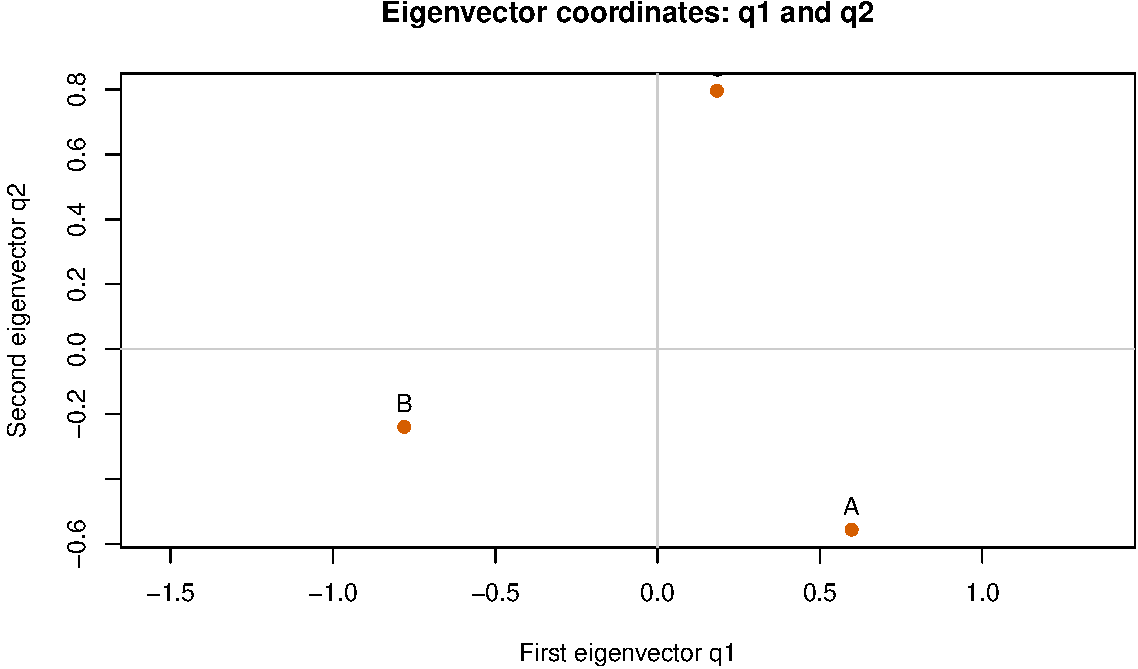
\includegraphics{11_mds_distances_files/figure-latex/spectral-step-3-1} \end{center}

\subsubsection{Step 4 --- recover
coordinates}\label{step-4-recover-coordinates}

Retain the \(r\) positive eigenvalues and their eigenvectors. If \(Q_r\)
and \(\Lambda_r\) are the retained matrices, the MDS coordinates are

\[X=Q_r\Lambda_r^{1/2}.\]

The recovered \(X\) can be translated, rotated or reflected relative to
X\_original; those transformations leave its distances unchanged.

\begin{Shaded}
\begin{Highlighting}[]
\NormalTok{positive }\OtherTok{\textless{}{-}} \FunctionTok{which}\NormalTok{(decomposition}\SpecialCharTok{$}\NormalTok{values }\SpecialCharTok{\textgreater{}} \DecValTok{1}\NormalTok{e}\SpecialCharTok{{-}}\DecValTok{10}\NormalTok{)}
\NormalTok{Q\_r }\OtherTok{\textless{}{-}}\NormalTok{ Q[, positive, drop }\OtherTok{=} \ConstantTok{FALSE}\NormalTok{]}
\NormalTok{Lambda\_r }\OtherTok{\textless{}{-}} \FunctionTok{diag}\NormalTok{(decomposition}\SpecialCharTok{$}\NormalTok{values[positive], }\AttributeTok{nrow =} \FunctionTok{length}\NormalTok{(positive))}
\NormalTok{X }\OtherTok{\textless{}{-}}\NormalTok{ Q\_r }\SpecialCharTok{\%*\%} \FunctionTok{sqrt}\NormalTok{(Lambda\_r)}
\FunctionTok{rownames}\NormalTok{(X) }\OtherTok{\textless{}{-}} \FunctionTok{rownames}\NormalTok{(D)}
\FunctionTok{colnames}\NormalTok{(X) }\OtherTok{\textless{}{-}} \FunctionTok{paste0}\NormalTok{(}\StringTok{"MDS"}\NormalTok{, }\FunctionTok{seq\_len}\NormalTok{(}\FunctionTok{ncol}\NormalTok{(X)))}

\NormalTok{X\_table }\OtherTok{\textless{}{-}} \FunctionTok{tibble}\NormalTok{(}\AttributeTok{object =} \FunctionTok{rownames}\NormalTok{(X), }\AttributeTok{MDS1 =}\NormalTok{ X[, }\DecValTok{1}\NormalTok{], }\AttributeTok{MDS2 =}\NormalTok{ X[, }\DecValTok{2}\NormalTok{])}
\NormalTok{knitr}\SpecialCharTok{::}\FunctionTok{kable}\NormalTok{(d\_orig, }\AttributeTok{digits =} \DecValTok{3}\NormalTok{, }\AttributeTok{caption =} \StringTok{"Step 4a: original coordinates d\_orig."}\NormalTok{)}
\end{Highlighting}
\end{Shaded}

\begin{longtable}[]{@{}lrr@{}}
\caption{Step 4a: original coordinates d\_orig.}\tabularnewline
\toprule\noalign{}
object & x & y \\
\midrule\noalign{}
\endfirsthead
\toprule\noalign{}
object & x & y \\
\midrule\noalign{}
\endhead
\bottomrule\noalign{}
\endlastfoot
A & 0 & 0 \\
B & 3 & 4 \\
C & 3 & 0 \\
\end{longtable}

\begin{Shaded}
\begin{Highlighting}[]
\NormalTok{knitr}\SpecialCharTok{::}\FunctionTok{kable}\NormalTok{(X\_table, }\AttributeTok{digits =} \DecValTok{3}\NormalTok{, }\AttributeTok{caption =} \StringTok{"Step 4b: coordinates X recovered by classical MDS."}\NormalTok{)}
\end{Highlighting}
\end{Shaded}

\begin{longtable}[]{@{}lrr@{}}
\caption{Step 4b: coordinates X recovered by classical
MDS.}\tabularnewline
\toprule\noalign{}
object & MDS1 & MDS2 \\
\midrule\noalign{}
\endfirsthead
\toprule\noalign{}
object & MDS1 & MDS2 \\
\midrule\noalign{}
\endhead
\bottomrule\noalign{}
\endlastfoot
A & 2.152 & -1.070 \\
B & -2.810 & -0.461 \\
C & 0.658 & 1.531 \\
\end{longtable}

\begin{Shaded}
\begin{Highlighting}[]
\NormalTok{old\_par }\OtherTok{\textless{}{-}} \FunctionTok{par}\NormalTok{(}\AttributeTok{no.readonly =} \ConstantTok{TRUE}\NormalTok{)}
\FunctionTok{par}\NormalTok{(}\AttributeTok{mfrow =} \FunctionTok{c}\NormalTok{(}\DecValTok{1}\NormalTok{, }\DecValTok{2}\NormalTok{), }\AttributeTok{mar =} \FunctionTok{c}\NormalTok{(}\DecValTok{4}\NormalTok{, }\DecValTok{4}\NormalTok{, }\DecValTok{3}\NormalTok{, }\DecValTok{1}\NormalTok{))}
\NormalTok{common\_limits }\OtherTok{\textless{}{-}} \FunctionTok{range}\NormalTok{(}\FunctionTok{c}\NormalTok{(d\_orig}\SpecialCharTok{$}\NormalTok{x, d\_orig}\SpecialCharTok{$}\NormalTok{y, X[, }\DecValTok{1}\NormalTok{], X[, }\DecValTok{2}\NormalTok{]))}
\NormalTok{common\_limits }\OtherTok{\textless{}{-}}\NormalTok{ common\_limits }\SpecialCharTok{+} \FunctionTok{c}\NormalTok{(}\SpecialCharTok{{-}}\FloatTok{.4}\NormalTok{, }\FloatTok{.4}\NormalTok{)}
\FunctionTok{plot}\NormalTok{(d\_orig}\SpecialCharTok{$}\NormalTok{x, d\_orig}\SpecialCharTok{$}\NormalTok{y, }\AttributeTok{asp =} \DecValTok{1}\NormalTok{, }\AttributeTok{pch =} \DecValTok{19}\NormalTok{, }\AttributeTok{col =}\NormalTok{ blue,}
     \AttributeTok{xlab =} \StringTok{"Coordinate 1"}\NormalTok{, }\AttributeTok{ylab =} \StringTok{"Coordinate 2"}\NormalTok{, }\AttributeTok{main =} \StringTok{"Original d\_orig"}\NormalTok{,}
     \AttributeTok{xlim =}\NormalTok{ common\_limits, }\AttributeTok{ylim =}\NormalTok{ common\_limits)}
\FunctionTok{text}\NormalTok{(d\_orig}\SpecialCharTok{$}\NormalTok{x, d\_orig}\SpecialCharTok{$}\NormalTok{y, }\AttributeTok{labels =}\NormalTok{ d\_orig}\SpecialCharTok{$}\NormalTok{object, }\AttributeTok{pos =} \DecValTok{3}\NormalTok{)}
\FunctionTok{plot}\NormalTok{(X[, }\DecValTok{1}\NormalTok{], X[, }\DecValTok{2}\NormalTok{], }\AttributeTok{asp =} \DecValTok{1}\NormalTok{, }\AttributeTok{pch =} \DecValTok{19}\NormalTok{, }\AttributeTok{col =}\NormalTok{ green,}
     \AttributeTok{xlab =} \StringTok{"MDS1"}\NormalTok{, }\AttributeTok{ylab =} \StringTok{"MDS2"}\NormalTok{, }\AttributeTok{main =} \StringTok{"Recovered X"}\NormalTok{,}
     \AttributeTok{xlim =}\NormalTok{ common\_limits, }\AttributeTok{ylim =}\NormalTok{ common\_limits)}
\FunctionTok{text}\NormalTok{(X[, }\DecValTok{1}\NormalTok{], X[, }\DecValTok{2}\NormalTok{], }\AttributeTok{labels =} \FunctionTok{rownames}\NormalTok{(X), }\AttributeTok{pos =} \DecValTok{3}\NormalTok{)}
\end{Highlighting}
\end{Shaded}

\begin{center}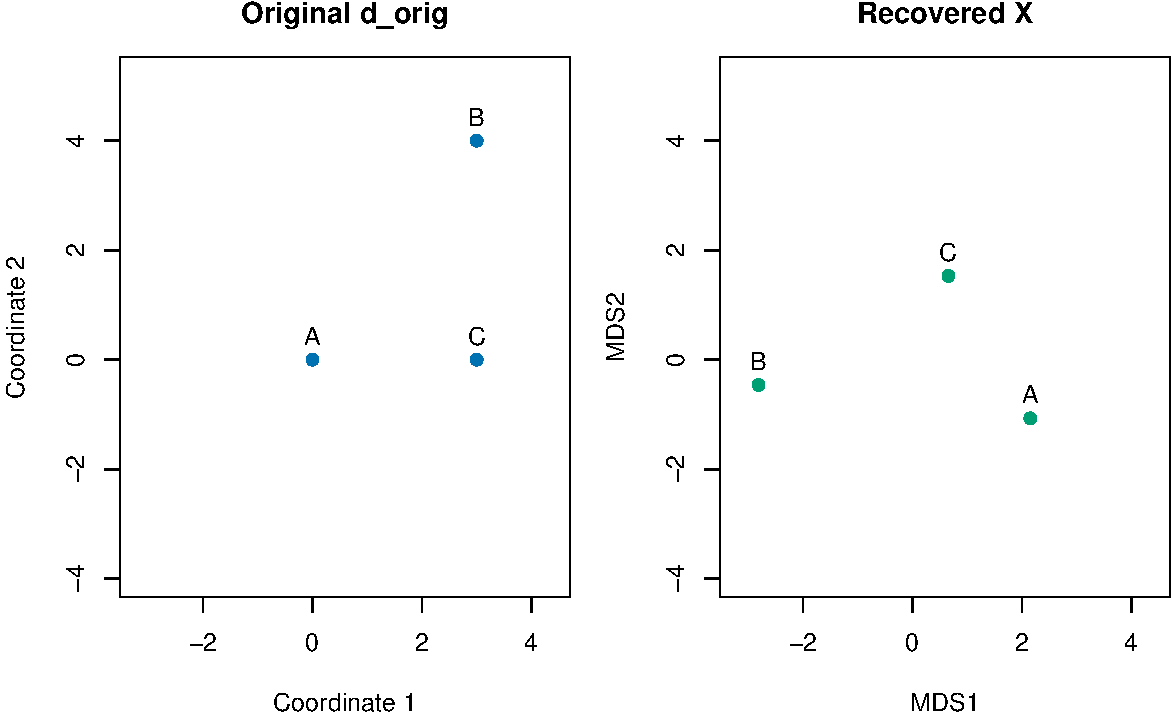
\includegraphics{11_mds_distances_files/figure-latex/spectral-step-4-1} \end{center}

\begin{Shaded}
\begin{Highlighting}[]
\FunctionTok{par}\NormalTok{(old\_par)}
\end{Highlighting}
\end{Shaded}

This is the whole classical-MDS mechanism. It is not a black box:
eigenvectors provide the coordinate directions, while eigenvalues
quantify how much centred squared-distance structure those directions
represent.

\subsection{The same objects in a reusable
function}\label{the-same-objects-in-a-reusable-function}

The function below uses the same names as the derivation: D, D2, J, B,
Q, Lambda and X. Its return value retains each object so that its
calculation can be inspected after fitting a larger dataset.

If B has a materially negative eigenvalue, its associated diagonal entry
in Lambda has no real square root. We therefore cannot turn that
component into real Euclidean coordinates. The function retains only
positive eigenvalues: its X is a Euclidean approximation, but it cannot
reconstruct the original D exactly when negative eigenvalues are
present.

\begin{Shaded}
\begin{Highlighting}[]
\NormalTok{classical\_mds }\OtherTok{\textless{}{-}} \ControlFlowTok{function}\NormalTok{(D, }\AttributeTok{k =} \DecValTok{2}\NormalTok{, }\AttributeTok{tolerance =} \DecValTok{1}\NormalTok{e}\SpecialCharTok{{-}}\DecValTok{10}\NormalTok{) \{}
\NormalTok{  D }\OtherTok{\textless{}{-}} \FunctionTok{as.matrix}\NormalTok{(D)}
\NormalTok{  D2 }\OtherTok{\textless{}{-}}\NormalTok{ D}\SpecialCharTok{\^{}}\DecValTok{2}
\NormalTok{  n }\OtherTok{\textless{}{-}} \FunctionTok{nrow}\NormalTok{(D)}
\NormalTok{  J }\OtherTok{\textless{}{-}} \FunctionTok{diag}\NormalTok{(n) }\SpecialCharTok{{-}} \FunctionTok{matrix}\NormalTok{(}\DecValTok{1} \SpecialCharTok{/}\NormalTok{ n, n, n)}
\NormalTok{  B }\OtherTok{\textless{}{-}} \SpecialCharTok{{-}}\FloatTok{0.5} \SpecialCharTok{*}\NormalTok{ J }\SpecialCharTok{\%*\%}\NormalTok{ D2 }\SpecialCharTok{\%*\%}\NormalTok{ J}

\NormalTok{  decomposition }\OtherTok{\textless{}{-}} \FunctionTok{eigen}\NormalTok{(B, }\AttributeTok{symmetric =} \ConstantTok{TRUE}\NormalTok{)}
\NormalTok{  Q }\OtherTok{\textless{}{-}}\NormalTok{ decomposition}\SpecialCharTok{$}\NormalTok{vectors}
\NormalTok{  Lambda }\OtherTok{\textless{}{-}} \FunctionTok{diag}\NormalTok{(decomposition}\SpecialCharTok{$}\NormalTok{values)}
\NormalTok{  positive }\OtherTok{\textless{}{-}} \FunctionTok{which}\NormalTok{(decomposition}\SpecialCharTok{$}\NormalTok{values }\SpecialCharTok{\textgreater{}}\NormalTok{ tolerance)}
\NormalTok{  keep }\OtherTok{\textless{}{-}}\NormalTok{ positive[}\FunctionTok{seq\_len}\NormalTok{(}\FunctionTok{min}\NormalTok{(k, }\FunctionTok{length}\NormalTok{(positive)))]}
\NormalTok{  Q\_r }\OtherTok{\textless{}{-}}\NormalTok{ Q[, keep, drop }\OtherTok{=} \ConstantTok{FALSE}\NormalTok{]}
\NormalTok{  Lambda\_r }\OtherTok{\textless{}{-}} \FunctionTok{diag}\NormalTok{(decomposition}\SpecialCharTok{$}\NormalTok{values[keep], }\AttributeTok{nrow =} \FunctionTok{length}\NormalTok{(keep))}
\NormalTok{  X }\OtherTok{\textless{}{-}}\NormalTok{ Q\_r }\SpecialCharTok{\%*\%} \FunctionTok{sqrt}\NormalTok{(Lambda\_r)}
  \FunctionTok{rownames}\NormalTok{(X) }\OtherTok{\textless{}{-}} \FunctionTok{rownames}\NormalTok{(D)}

  \FunctionTok{list}\NormalTok{(}\AttributeTok{D =}\NormalTok{ D, }\AttributeTok{D2 =}\NormalTok{ D2, }\AttributeTok{J =}\NormalTok{ J, }\AttributeTok{B =}\NormalTok{ B, }\AttributeTok{Q =}\NormalTok{ Q, }\AttributeTok{Lambda =}\NormalTok{ Lambda,}
       \AttributeTok{X =}\NormalTok{ X, }\AttributeTok{eigenvalues =}\NormalTok{ decomposition}\SpecialCharTok{$}\NormalTok{values)}
\NormalTok{\}}

\NormalTok{mds\_bray }\OtherTok{\textless{}{-}} \FunctionTok{classical\_mds}\NormalTok{(d\_bray, }\AttributeTok{k =} \DecValTok{2}\NormalTok{)}
\NormalTok{mds\_hellinger }\OtherTok{\textless{}{-}} \FunctionTok{classical\_mds}\NormalTok{(d\_hellinger, }\AttributeTok{k =} \DecValTok{2}\NormalTok{)}
\FunctionTok{round}\NormalTok{(mds\_bray}\SpecialCharTok{$}\NormalTok{eigenvalues, }\DecValTok{4}\NormalTok{)}
\end{Highlighting}
\end{Shaded}

\begin{verbatim}
#>  [1]  1.7163  1.0224  0.4615  0.3822  0.2791  0.2366  0.1691  0.0962  0.0745
#> [10]  0.0617  0.0549  0.0192  0.0161  0.0040  0.0000 -0.0264 -0.0429 -0.0547
#> [19] -0.0741 -0.0968
\end{verbatim}

\subsection{MDS map of the
communities}\label{mds-map-of-the-communities}

\begin{Shaded}
\begin{Highlighting}[]
\NormalTok{mds\_df }\OtherTok{\textless{}{-}} \FunctionTok{as.data.frame}\NormalTok{(mds\_bray}\SpecialCharTok{$}\NormalTok{X) }\SpecialCharTok{|\textgreater{}}
  \FunctionTok{setNames}\NormalTok{(}\FunctionTok{c}\NormalTok{(}\StringTok{"MDS1"}\NormalTok{, }\StringTok{"MDS2"}\NormalTok{)) }\SpecialCharTok{|\textgreater{}}
  \FunctionTok{mutate}\NormalTok{(}\AttributeTok{site =} \FunctionTok{rownames}\NormalTok{(mds\_bray}\SpecialCharTok{$}\NormalTok{X)) }\SpecialCharTok{|\textgreater{}}
  \FunctionTok{left\_join}\NormalTok{(site\_metadata }\SpecialCharTok{|\textgreater{}} \FunctionTok{select}\NormalTok{(site, Management, Moisture), }\AttributeTok{by =} \StringTok{"site"}\NormalTok{)}

\FunctionTok{ggplot}\NormalTok{(mds\_df, }\FunctionTok{aes}\NormalTok{(MDS1, MDS2, }\AttributeTok{colour =}\NormalTok{ Management, }\AttributeTok{label =}\NormalTok{ site)) }\SpecialCharTok{+}
  \FunctionTok{geom\_hline}\NormalTok{(}\AttributeTok{yintercept =} \DecValTok{0}\NormalTok{, }\AttributeTok{colour =} \StringTok{"grey85"}\NormalTok{) }\SpecialCharTok{+}
  \FunctionTok{geom\_vline}\NormalTok{(}\AttributeTok{xintercept =} \DecValTok{0}\NormalTok{, }\AttributeTok{colour =} \StringTok{"grey85"}\NormalTok{) }\SpecialCharTok{+}
  \FunctionTok{geom\_point}\NormalTok{(}\AttributeTok{size =} \DecValTok{4}\NormalTok{) }\SpecialCharTok{+}
  \FunctionTok{geom\_text}\NormalTok{(}\AttributeTok{nudge\_y =} \FloatTok{0.025}\NormalTok{, }\AttributeTok{show.legend =} \ConstantTok{FALSE}\NormalTok{) }\SpecialCharTok{+}
  \FunctionTok{scale\_colour\_brewer}\NormalTok{(}\AttributeTok{palette =} \StringTok{"Dark2"}\NormalTok{) }\SpecialCharTok{+}
  \FunctionTok{coord\_equal}\NormalTok{() }\SpecialCharTok{+}
  \FunctionTok{labs}\NormalTok{(}\AttributeTok{title =} \StringTok{"Community composition: Bray{-}{-}Curtis MDS"}\NormalTok{, }\AttributeTok{x =} \StringTok{"MDS dimension 1"}\NormalTok{, }\AttributeTok{y =} \StringTok{"MDS dimension 2"}\NormalTok{, }\AttributeTok{colour =} \StringTok{"Management"}\NormalTok{)}
\end{Highlighting}
\end{Shaded}

\begin{figure}

{\centering 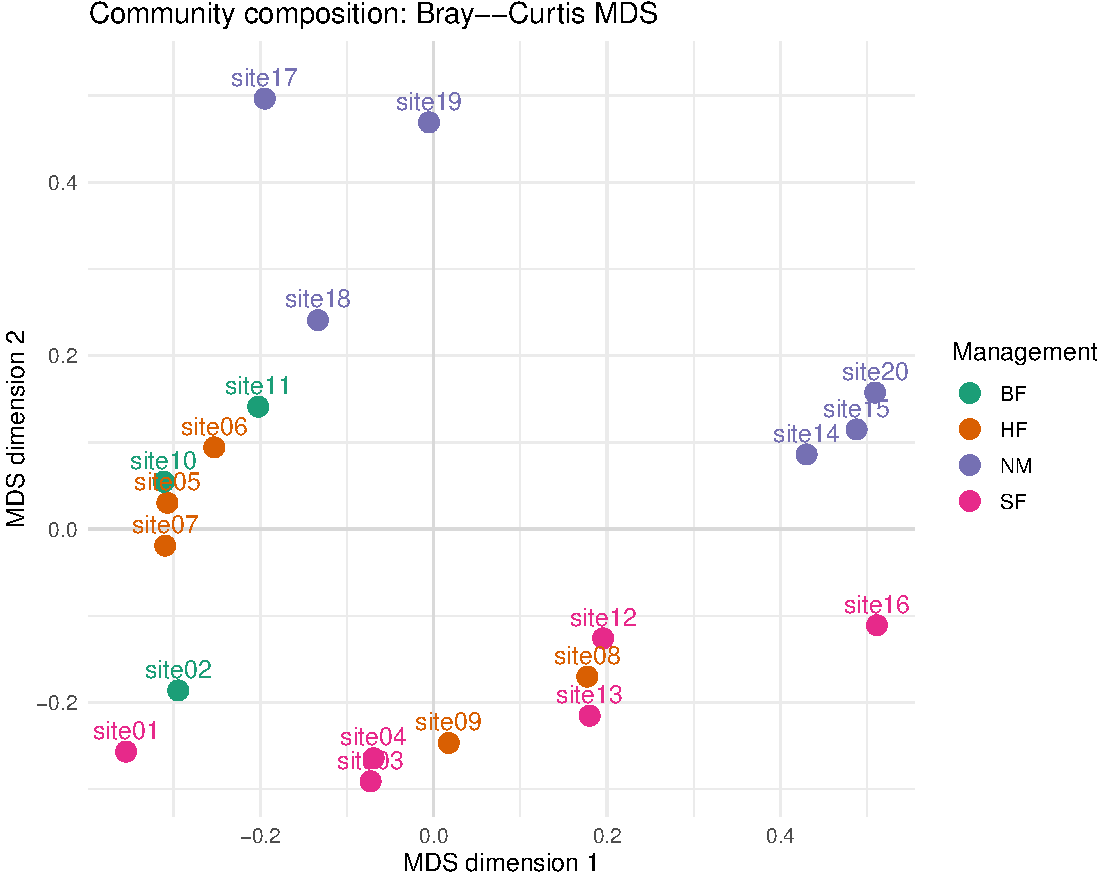
\includegraphics{11_mds_distances_files/figure-latex/bray-mds-map-1} 

}

\caption{Classical MDS map based on Bray--Curtis dissimilarity. Colour records the observed management category; the map itself was computed using species cover classes only.}\label{fig:bray-mds-map}
\end{figure}

Sites with similar species composition tend to lie close together;
management is shown as external descriptive context, not as an input to
the distance. Any visual association with management is exploratory and
does not establish a causal effect.

\subsection{Why MDS axes have no inherent
interpretation}\label{why-mds-axes-have-no-inherent-interpretation}

Multiplying every coordinate matrix by an orthogonal rotation or
reflection leaves all interpoint Euclidean distances unchanged. Thus
MDS1 is not ``the management gradient'' unless an external analysis
supports that interpretation. The stable evidence is proximity,
separation, groups and the fit of map distances to original distances.

\begin{Shaded}
\begin{Highlighting}[]
\NormalTok{rot90 }\OtherTok{\textless{}{-}} \FunctionTok{matrix}\NormalTok{(}\FunctionTok{c}\NormalTok{(}\DecValTok{0}\NormalTok{, }\SpecialCharTok{{-}}\DecValTok{1}\NormalTok{, }\DecValTok{1}\NormalTok{, }\DecValTok{0}\NormalTok{), }\AttributeTok{nrow =} \DecValTok{2}\NormalTok{)}
\NormalTok{rotated }\OtherTok{\textless{}{-}} \FunctionTok{as.matrix}\NormalTok{(mds\_df[, }\FunctionTok{c}\NormalTok{(}\StringTok{"MDS1"}\NormalTok{, }\StringTok{"MDS2"}\NormalTok{)]) }\SpecialCharTok{\%*\%}\NormalTok{ rot90}
\NormalTok{rotated\_df }\OtherTok{\textless{}{-}} \FunctionTok{data.frame}\NormalTok{(}\AttributeTok{MDS1 =}\NormalTok{ rotated[, }\DecValTok{1}\NormalTok{], }\AttributeTok{MDS2 =}\NormalTok{ rotated[, }\DecValTok{2}\NormalTok{], }\AttributeTok{site =}\NormalTok{ mds\_df}\SpecialCharTok{$}\NormalTok{site, }\AttributeTok{Management =}\NormalTok{ mds\_df}\SpecialCharTok{$}\NormalTok{Management)}

\NormalTok{p1 }\OtherTok{\textless{}{-}} \FunctionTok{ggplot}\NormalTok{(mds\_df, }\FunctionTok{aes}\NormalTok{(MDS1, MDS2, }\AttributeTok{colour =}\NormalTok{ Management, }\AttributeTok{label =}\NormalTok{ site)) }\SpecialCharTok{+} \FunctionTok{geom\_point}\NormalTok{(}\AttributeTok{size =} \DecValTok{3}\NormalTok{) }\SpecialCharTok{+} \FunctionTok{geom\_text}\NormalTok{(}\AttributeTok{nudge\_y =} \FloatTok{.025}\NormalTok{) }\SpecialCharTok{+} \FunctionTok{coord\_equal}\NormalTok{() }\SpecialCharTok{+} \FunctionTok{labs}\NormalTok{(}\AttributeTok{title =} \StringTok{"Original orientation"}\NormalTok{)}
\NormalTok{p2 }\OtherTok{\textless{}{-}} \FunctionTok{ggplot}\NormalTok{(rotated\_df, }\FunctionTok{aes}\NormalTok{(MDS1, MDS2, }\AttributeTok{colour =}\NormalTok{ Management, }\AttributeTok{label =}\NormalTok{ site)) }\SpecialCharTok{+} \FunctionTok{geom\_point}\NormalTok{(}\AttributeTok{size =} \DecValTok{3}\NormalTok{) }\SpecialCharTok{+} \FunctionTok{geom\_text}\NormalTok{(}\AttributeTok{nudge\_y =} \FloatTok{.025}\NormalTok{) }\SpecialCharTok{+} \FunctionTok{coord\_equal}\NormalTok{() }\SpecialCharTok{+} \FunctionTok{labs}\NormalTok{(}\AttributeTok{title =} \StringTok{"Rotated orientation"}\NormalTok{)}

\FunctionTok{print}\NormalTok{(p1)}
\end{Highlighting}
\end{Shaded}

\begin{figure}

{\centering 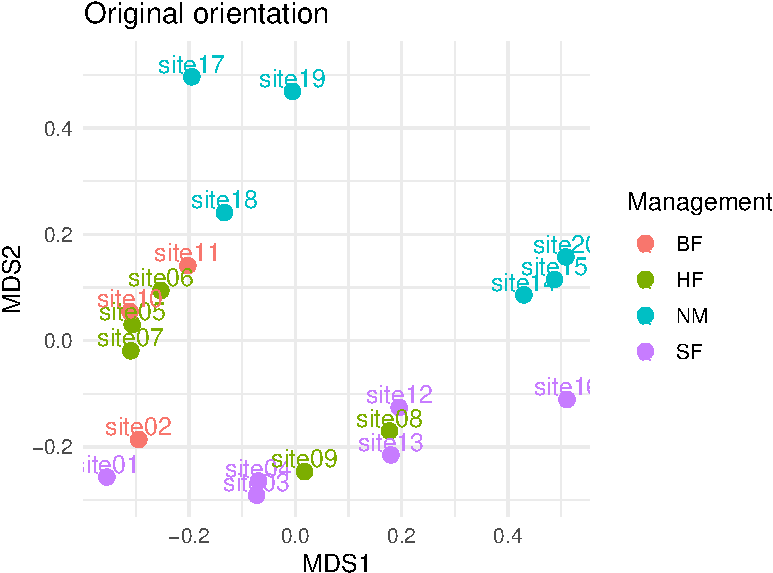
\includegraphics{11_mds_distances_files/figure-latex/rotation-invariance-1} 

}

\caption{A 90-degree rotation changes axes but preserves all pairwise distances. Both panels are the same MDS solution.}\label{fig:rotation-invariance-1}
\end{figure}

\begin{Shaded}
\begin{Highlighting}[]
\FunctionTok{print}\NormalTok{(p2)}
\end{Highlighting}
\end{Shaded}

\begin{figure}

{\centering 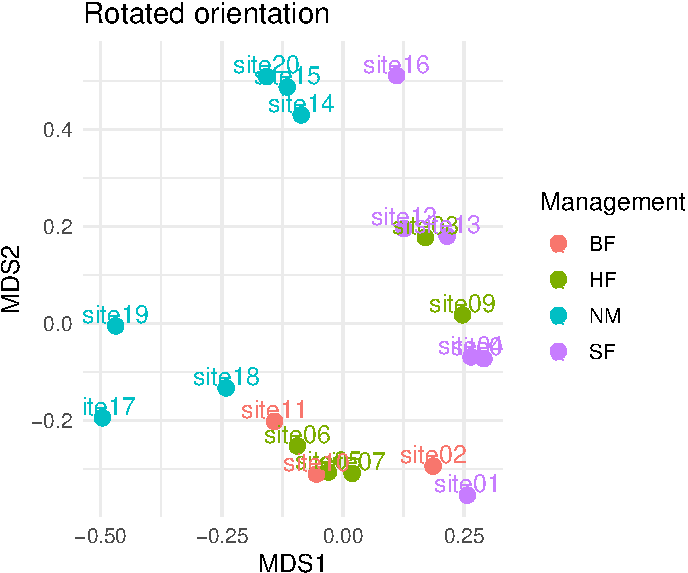
\includegraphics{11_mds_distances_files/figure-latex/rotation-invariance-2} 

}

\caption{A 90-degree rotation changes axes but preserves all pairwise distances. Both panels are the same MDS solution.}\label{fig:rotation-invariance-2}
\end{figure}

\section{Choosing the number of
dimensions}\label{choosing-the-number-of-dimensions}

Two dimensions are chosen here because the intended final display is a
static map. This is a communication constraint, not evidence that the
data are intrinsically two-dimensional. In an exactly Euclidean problem,
the number of positive eigenvalues is the dimension required for exact
reconstruction. With non-Euclidean dissimilarities, negative eigenvalues
add a separate warning about the geometry.

Choose \(k\) using all three pieces of evidence below:

\begin{enumerate}
\def\labelenumi{\arabic{enumi}.}
\tightlist
\item
  \textbf{Eigenvalue spectrum:} is there an elbow after the first few
  positive eigenvalues?
\item
  \textbf{Distance reproduction:} does the configuration preserve the
  pairwise distances sufficiently for the intended claim?
\item
  \textbf{Communication purpose:} two dimensions are easy to print and
  annotate; three dimensions may be inspected interactively; additional
  dimensions may be retained for later analysis without being drawn as a
  single map.
\end{enumerate}

Do not call the eigenvalue fraction ``variance explained'' without
qualification: this is MDS of a distance matrix, not PCA of the original
variables. Here we use the fraction of \textbf{absolute-eigenvalue
structure}. Its denominator is \(\sum_j|\lambda_j|\), including negative
eigenvalues. Thus even retaining every positive eigenvalue need not
reach 100\%: the remaining fraction is non-Euclidean structure that no
real Euclidean coordinate system can reproduce exactly.

\begin{Shaded}
\begin{Highlighting}[]
\NormalTok{positive\_bray }\OtherTok{\textless{}{-}}\NormalTok{ mds\_bray}\SpecialCharTok{$}\NormalTok{eigenvalues[mds\_bray}\SpecialCharTok{$}\NormalTok{eigenvalues }\SpecialCharTok{\textgreater{}} \DecValTok{1}\NormalTok{e}\SpecialCharTok{{-}}\DecValTok{10}\NormalTok{]}
\NormalTok{total\_absolute\_structure }\OtherTok{\textless{}{-}} \FunctionTok{sum}\NormalTok{(}\FunctionTok{abs}\NormalTok{(mds\_bray}\SpecialCharTok{$}\NormalTok{eigenvalues))}
\NormalTok{negative\_structure\_fraction }\OtherTok{\textless{}{-}} \FunctionTok{sum}\NormalTok{(}\FunctionTok{abs}\NormalTok{(mds\_bray}\SpecialCharTok{$}\NormalTok{eigenvalues[mds\_bray}\SpecialCharTok{$}\NormalTok{eigenvalues }\SpecialCharTok{\textless{}} \SpecialCharTok{{-}}\DecValTok{1}\NormalTok{e}\SpecialCharTok{{-}}\DecValTok{10}\NormalTok{])) }\SpecialCharTok{/}
\NormalTok{  total\_absolute\_structure}
\NormalTok{dimension\_summary }\OtherTok{\textless{}{-}} \FunctionTok{tibble}\NormalTok{(}
  \AttributeTok{dimension =} \FunctionTok{seq\_along}\NormalTok{(positive\_bray),}
  \AttributeTok{eigenvalue =}\NormalTok{ positive\_bray,}
  \AttributeTok{cumulative\_fraction =} \FunctionTok{cumsum}\NormalTok{(positive\_bray) }\SpecialCharTok{/}\NormalTok{ total\_absolute\_structure}
\NormalTok{)}

\NormalTok{p\_scree }\OtherTok{\textless{}{-}} \FunctionTok{ggplot}\NormalTok{(dimension\_summary, }\FunctionTok{aes}\NormalTok{(dimension, eigenvalue)) }\SpecialCharTok{+}
  \FunctionTok{geom\_col}\NormalTok{(}\AttributeTok{fill =}\NormalTok{ blue) }\SpecialCharTok{+}
  \FunctionTok{labs}\NormalTok{(}\AttributeTok{title =} \StringTok{"Positive{-}eigenvalue spectrum"}\NormalTok{, }\AttributeTok{x =} \StringTok{"Dimension"}\NormalTok{, }\AttributeTok{y =} \StringTok{"Eigenvalue"}\NormalTok{)}

\NormalTok{p\_cumulative }\OtherTok{\textless{}{-}} \FunctionTok{ggplot}\NormalTok{(dimension\_summary, }\FunctionTok{aes}\NormalTok{(dimension, cumulative\_fraction)) }\SpecialCharTok{+}
  \FunctionTok{geom\_line}\NormalTok{(}\AttributeTok{colour =}\NormalTok{ orange, }\AttributeTok{linewidth =} \DecValTok{1}\NormalTok{) }\SpecialCharTok{+}
  \FunctionTok{geom\_point}\NormalTok{(}\AttributeTok{colour =}\NormalTok{ orange, }\AttributeTok{size =} \FloatTok{2.5}\NormalTok{) }\SpecialCharTok{+}
  \FunctionTok{scale\_y\_continuous}\NormalTok{(}\AttributeTok{labels =}\NormalTok{ scales}\SpecialCharTok{::}\FunctionTok{percent\_format}\NormalTok{(}\AttributeTok{accuracy =} \DecValTok{1}\NormalTok{), }\AttributeTok{limits =} \FunctionTok{c}\NormalTok{(}\DecValTok{0}\NormalTok{, }\DecValTok{1}\NormalTok{)) }\SpecialCharTok{+}
  \FunctionTok{labs}\NormalTok{(}\AttributeTok{title =} \StringTok{"Cumulative absolute{-}eigenvalue fraction"}\NormalTok{, }\AttributeTok{x =} \StringTok{"Dimensions retained"}\NormalTok{,}
       \AttributeTok{y =} \StringTok{"Fraction of total absolute structure"}\NormalTok{)}

\FunctionTok{print}\NormalTok{(p\_scree)}
\end{Highlighting}
\end{Shaded}

\begin{figure}

{\centering 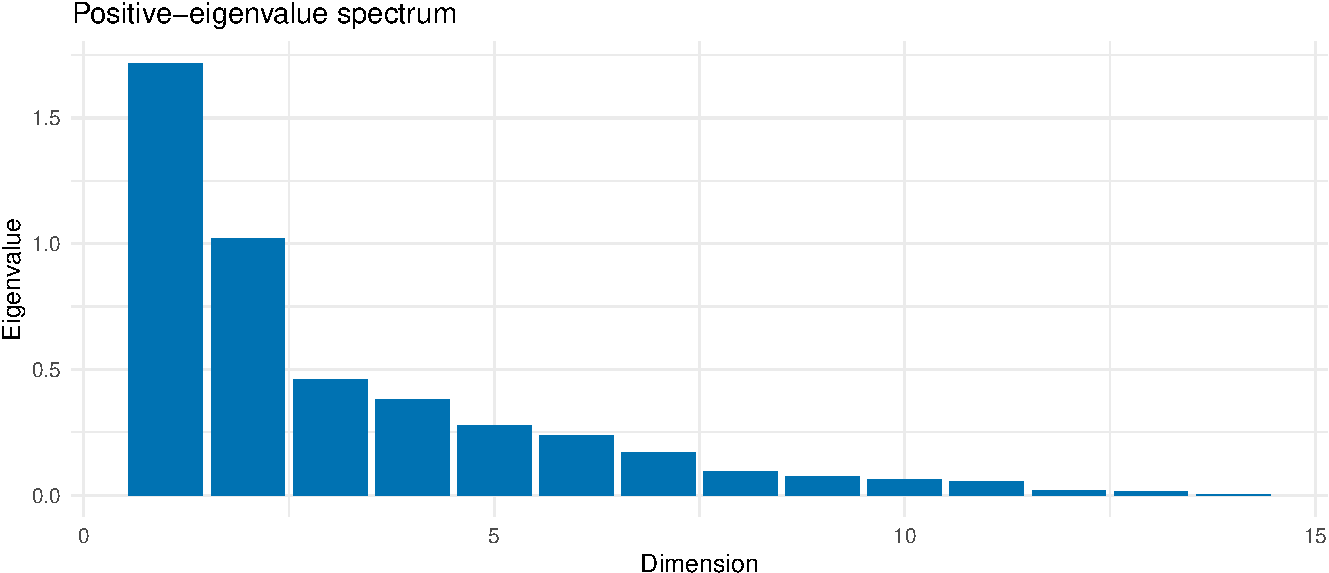
\includegraphics{11_mds_distances_files/figure-latex/choose-dimensions-1} 

}

\caption{The positive-eigenvalue scree plot and the cumulative absolute-eigenvalue fraction separate represented Euclidean structure from non-Euclidean structure.}\label{fig:choose-dimensions-1}
\end{figure}

\begin{Shaded}
\begin{Highlighting}[]
\FunctionTok{print}\NormalTok{(p\_cumulative)}
\end{Highlighting}
\end{Shaded}

\begin{figure}

{\centering 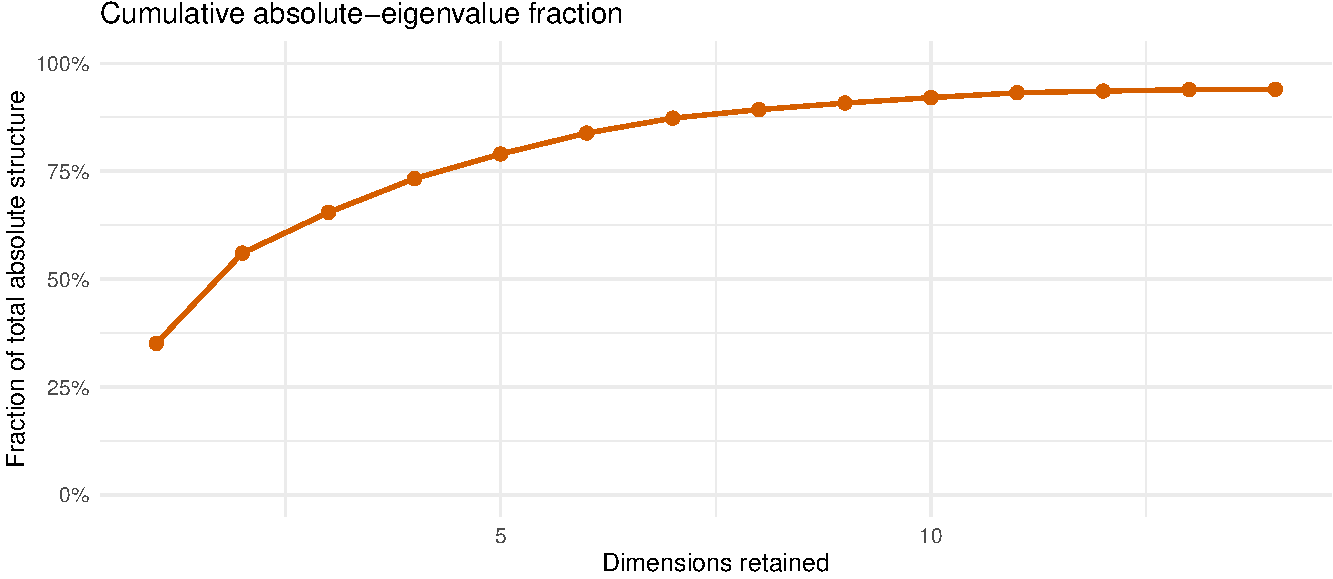
\includegraphics{11_mds_distances_files/figure-latex/choose-dimensions-2} 

}

\caption{The positive-eigenvalue scree plot and the cumulative absolute-eigenvalue fraction separate represented Euclidean structure from non-Euclidean structure.}\label{fig:choose-dimensions-2}
\end{figure}

\begin{Shaded}
\begin{Highlighting}[]
\NormalTok{scales}\SpecialCharTok{::}\FunctionTok{percent}\NormalTok{(negative\_structure\_fraction, }\AttributeTok{accuracy =} \FloatTok{.1}\NormalTok{)}
\end{Highlighting}
\end{Shaded}

\begin{verbatim}
#> [1] "6.0%"
\end{verbatim}

The printed percentage is the share of total absolute-eigenvalue
structure carried by negative eigenvalues. It is the portion that will
remain unreconstructable in any real Euclidean MDS configuration,
regardless of how many positive dimensions are retained.

\section{Reading MDS eigenvalues and
fit}\label{reading-mds-eigenvalues-and-fit}

For an exactly Euclidean distance, all non-zero eigenvalues of \(B\) are
non-negative. Bray--Curtis is not guaranteed to have that property.
Small negative eigenvalues tell us that no exact Euclidean configuration
reproduces all of its distances. They are not an automatic failure: they
are diagnostic evidence that the distance geometry is only approximately
Euclidean.

\begin{Shaded}
\begin{Highlighting}[]
\NormalTok{eig\_df }\OtherTok{\textless{}{-}} \FunctionTok{tibble}\NormalTok{(}\AttributeTok{dimension =} \FunctionTok{seq\_along}\NormalTok{(mds\_bray}\SpecialCharTok{$}\NormalTok{eigenvalues), }\AttributeTok{eigenvalue =}\NormalTok{ mds\_bray}\SpecialCharTok{$}\NormalTok{eigenvalues)}
\FunctionTok{ggplot}\NormalTok{(eig\_df, }\FunctionTok{aes}\NormalTok{(dimension, eigenvalue, }\AttributeTok{fill =}\NormalTok{ eigenvalue }\SpecialCharTok{\textgreater{}} \DecValTok{0}\NormalTok{)) }\SpecialCharTok{+}
  \FunctionTok{geom\_col}\NormalTok{(}\AttributeTok{show.legend =} \ConstantTok{FALSE}\NormalTok{) }\SpecialCharTok{+}
  \FunctionTok{geom\_hline}\NormalTok{(}\AttributeTok{yintercept =} \DecValTok{0}\NormalTok{) }\SpecialCharTok{+}
  \FunctionTok{scale\_fill\_manual}\NormalTok{(}\AttributeTok{values =} \FunctionTok{c}\NormalTok{(}\StringTok{\textasciigrave{}}\AttributeTok{TRUE}\StringTok{\textasciigrave{}} \OtherTok{=}\NormalTok{ blue, }\StringTok{\textasciigrave{}}\AttributeTok{FALSE}\StringTok{\textasciigrave{}} \OtherTok{=}\NormalTok{ orange)) }\SpecialCharTok{+}
  \FunctionTok{labs}\NormalTok{(}\AttributeTok{title =} \StringTok{"MDS eigenvalues"}\NormalTok{, }\AttributeTok{x =} \StringTok{"Dimension"}\NormalTok{, }\AttributeTok{y =} \StringTok{"Eigenvalue"}\NormalTok{)}
\end{Highlighting}
\end{Shaded}

\begin{figure}

{\centering 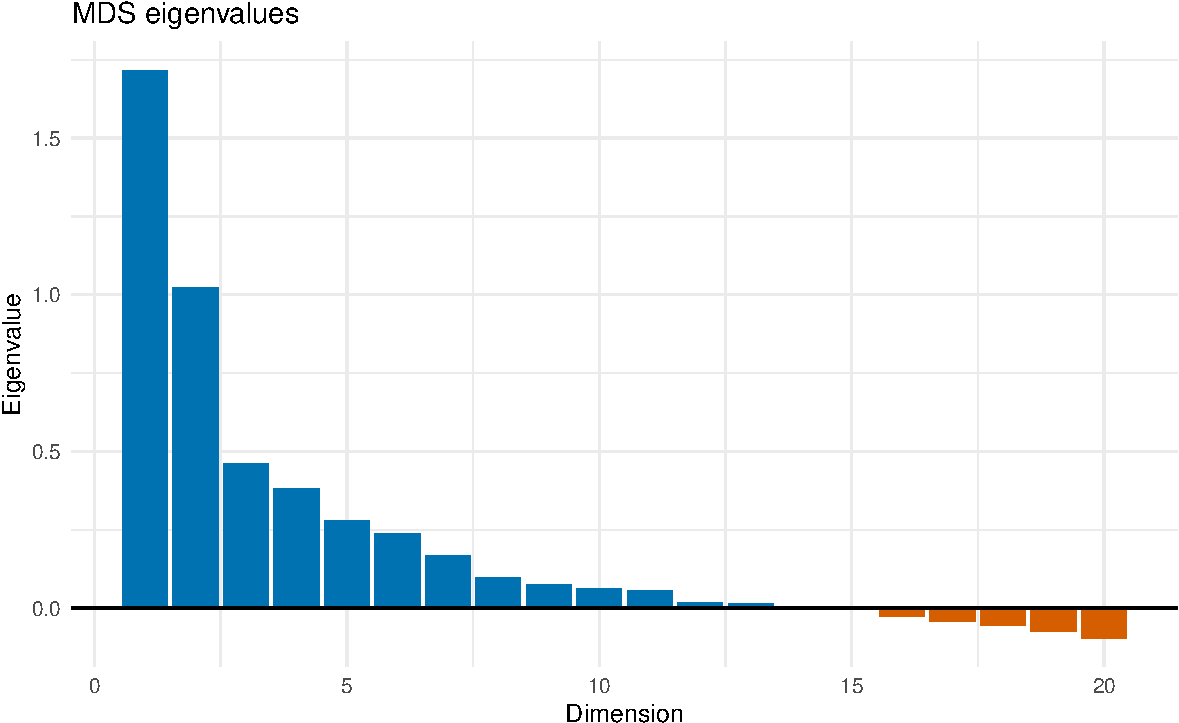
\includegraphics{11_mds_distances_files/figure-latex/eigenvalue-plot-1} 

}

\caption{Positive and negative MDS eigenvalues for Bray--Curtis dissimilarity. Negative values reveal non-Euclidean structure.}\label{fig:eigenvalue-plot}
\end{figure}

Two simple summaries are useful:

\begin{Shaded}
\begin{Highlighting}[]
\NormalTok{abs\_eigen }\OtherTok{\textless{}{-}} \FunctionTok{abs}\NormalTok{(mds\_bray}\SpecialCharTok{$}\NormalTok{eigenvalues)}
\NormalTok{variance\_like\_fit }\OtherTok{\textless{}{-}} \FunctionTok{sum}\NormalTok{(abs\_eigen[}\DecValTok{1}\SpecialCharTok{:}\DecValTok{2}\NormalTok{]) }\SpecialCharTok{/} \FunctionTok{sum}\NormalTok{(abs\_eigen)}

\NormalTok{map\_d }\OtherTok{\textless{}{-}} \FunctionTok{dist}\NormalTok{(mds\_bray}\SpecialCharTok{$}\NormalTok{X)}
\NormalTok{distance\_correlation }\OtherTok{\textless{}{-}} \FunctionTok{cor}\NormalTok{(}\FunctionTok{as.vector}\NormalTok{(d\_bray), }\FunctionTok{as.vector}\NormalTok{(map\_d))}

\FunctionTok{c}\NormalTok{(}\AttributeTok{two\_dimension\_positive\_eigenvalue\_fraction =}\NormalTok{ variance\_like\_fit,}
  \AttributeTok{correlation\_original\_vs\_map\_distance =}\NormalTok{ distance\_correlation)}
\end{Highlighting}
\end{Shaded}

\begin{verbatim}
#> two_dimension_positive_eigenvalue_fraction 
#>                                  0.5601833 
#>       correlation_original_vs_map_distance 
#>                                  0.9163764
\end{verbatim}

The first value reports how much of the \textbf{absolute-eigenvalue}
structure is retained in two dimensions. The overall structure comprises
the positive eigenvalues that can be represented in an Euclidean space
(i.e.~by increasing the number of dimensions), and the negative ones
that cannot be described by an Euclidean distance, no matter the number
of dimensions. The second reports whether pairs far apart in the
original distance also tend to be far apart on the map. Neither is a
universal threshold; inspect the map and its distance reproduction
before treating it as a complete representation.

\subsection{What changes under Hellinger--Euclidean
distance?}\label{what-changes-under-hellingereuclidean-distance}

The following comparison does not select a winner mechanically. It makes
the trade-off explicit: Bray--Curtis is a familiar ecological
dissimilarity but its classical MDS has negative eigenvalues;
Hellinger--Euclidean distance gives an exactly Euclidean input but can
emphasise a different ecological contrast.

\begin{Shaded}
\begin{Highlighting}[]
\NormalTok{mds\_summary }\OtherTok{\textless{}{-}} \ControlFlowTok{function}\NormalTok{(d, fit) \{}
\NormalTok{  eig }\OtherTok{\textless{}{-}}\NormalTok{ fit}\SpecialCharTok{$}\NormalTok{eigenvalues}
\NormalTok{  total\_absolute\_structure }\OtherTok{\textless{}{-}} \FunctionTok{sum}\NormalTok{(}\FunctionTok{abs}\NormalTok{(eig))}
\NormalTok{  retained\_absolute\_structure }\OtherTok{\textless{}{-}} \FunctionTok{sum}\NormalTok{(}\FunctionTok{abs}\NormalTok{(eig[}\FunctionTok{seq\_len}\NormalTok{(}\FunctionTok{min}\NormalTok{(}\DecValTok{2}\NormalTok{, }\FunctionTok{length}\NormalTok{(eig)))]))}
\NormalTok{  map\_distance }\OtherTok{\textless{}{-}} \FunctionTok{dist}\NormalTok{(fit}\SpecialCharTok{$}\NormalTok{X)}
  \FunctionTok{c}\NormalTok{(}
    \AttributeTok{negative\_eigenvalues =} \FunctionTok{sum}\NormalTok{(eig }\SpecialCharTok{\textless{}} \SpecialCharTok{{-}}\DecValTok{1}\NormalTok{e}\SpecialCharTok{{-}}\DecValTok{10}\NormalTok{),}
    \AttributeTok{negative\_absolute\_fraction =} \FunctionTok{sum}\NormalTok{(}\FunctionTok{abs}\NormalTok{(eig[eig }\SpecialCharTok{\textless{}} \SpecialCharTok{{-}}\DecValTok{1}\NormalTok{e}\SpecialCharTok{{-}}\DecValTok{10}\NormalTok{])) }\SpecialCharTok{/}\NormalTok{ total\_absolute\_structure,}
    \AttributeTok{two\_dimension\_absolute\_fraction =}\NormalTok{ retained\_absolute\_structure }\SpecialCharTok{/}\NormalTok{ total\_absolute\_structure,}
    \AttributeTok{original\_map\_distance\_correlation =} \FunctionTok{cor}\NormalTok{(}\FunctionTok{as.vector}\NormalTok{(d), }\FunctionTok{as.vector}\NormalTok{(map\_distance))}
\NormalTok{  )}
\NormalTok{\}}

\NormalTok{comparison\_table }\OtherTok{\textless{}{-}} \FunctionTok{rbind}\NormalTok{(}
  \StringTok{\textasciigrave{}}\AttributeTok{Bray{-}{-}Curtis}\StringTok{\textasciigrave{}} \OtherTok{=} \FunctionTok{mds\_summary}\NormalTok{(d\_bray, mds\_bray),}
  \StringTok{\textasciigrave{}}\AttributeTok{Hellinger + Euclidean}\StringTok{\textasciigrave{}} \OtherTok{=} \FunctionTok{mds\_summary}\NormalTok{(d\_hellinger, mds\_hellinger)}
\NormalTok{)}
\NormalTok{knitr}\SpecialCharTok{::}\FunctionTok{kable}\NormalTok{(}\FunctionTok{round}\NormalTok{(comparison\_table, }\DecValTok{3}\NormalTok{), }\AttributeTok{caption =} \StringTok{"Diagnostics for two defensible distance choices. Higher map{-}distance correlation indicates better two{-}dimensional distance reproduction; it is not a universal measure of scientific quality."}\NormalTok{)}
\end{Highlighting}
\end{Shaded}

\begin{longtable}[]{@{}
  >{\raggedright\arraybackslash}p{(\linewidth - 8\tabcolsep) * \real{0.1618}}
  >{\raggedleft\arraybackslash}p{(\linewidth - 8\tabcolsep) * \real{0.1544}}
  >{\raggedleft\arraybackslash}p{(\linewidth - 8\tabcolsep) * \real{0.1985}}
  >{\raggedleft\arraybackslash}p{(\linewidth - 8\tabcolsep) * \real{0.2353}}
  >{\raggedleft\arraybackslash}p{(\linewidth - 8\tabcolsep) * \real{0.2500}}@{}}
\caption{Diagnostics for two defensible distance choices. Higher
map-distance correlation indicates better two-dimensional distance
reproduction; it is not a universal measure of scientific
quality.}\tabularnewline
\toprule\noalign{}
\begin{minipage}[b]{\linewidth}\raggedright
\end{minipage} & \begin{minipage}[b]{\linewidth}\raggedleft
negative\_eigenvalues
\end{minipage} & \begin{minipage}[b]{\linewidth}\raggedleft
negative\_absolute\_fraction
\end{minipage} & \begin{minipage}[b]{\linewidth}\raggedleft
two\_dimension\_absolute\_fraction
\end{minipage} & \begin{minipage}[b]{\linewidth}\raggedleft
original\_map\_distance\_correlation
\end{minipage} \\
\midrule\noalign{}
\endfirsthead
\toprule\noalign{}
\begin{minipage}[b]{\linewidth}\raggedright
\end{minipage} & \begin{minipage}[b]{\linewidth}\raggedleft
negative\_eigenvalues
\end{minipage} & \begin{minipage}[b]{\linewidth}\raggedleft
negative\_absolute\_fraction
\end{minipage} & \begin{minipage}[b]{\linewidth}\raggedleft
two\_dimension\_absolute\_fraction
\end{minipage} & \begin{minipage}[b]{\linewidth}\raggedleft
original\_map\_distance\_correlation
\end{minipage} \\
\midrule\noalign{}
\endhead
\bottomrule\noalign{}
\endlastfoot
Bray--Curtis & 5 & 0.06 & 0.560 & 0.916 \\
Hellinger + Euclidean & 0 & 0.00 & 0.505 & 0.905 \\
\end{longtable}

If the scientific message is stable across the two maps, confidence in
the broad description increases. If it changes, do not choose the
prettier map: return to the data-generating and sampling context, state
the competing definitions of similarity, and report the sensitivity.

\begin{Shaded}
\begin{Highlighting}[]
\NormalTok{shepard }\OtherTok{\textless{}{-}} \FunctionTok{tibble}\NormalTok{(}\AttributeTok{original =} \FunctionTok{as.vector}\NormalTok{(d\_bray), }\AttributeTok{map =} \FunctionTok{as.vector}\NormalTok{(map\_d))}
\FunctionTok{ggplot}\NormalTok{(shepard, }\FunctionTok{aes}\NormalTok{(original, map)) }\SpecialCharTok{+}
  \FunctionTok{geom\_point}\NormalTok{(}\AttributeTok{size =} \FloatTok{2.5}\NormalTok{, }\AttributeTok{colour =}\NormalTok{ blue, }\AttributeTok{alpha =} \FloatTok{.8}\NormalTok{) }\SpecialCharTok{+}
  \FunctionTok{geom\_abline}\NormalTok{(}\AttributeTok{slope =} \DecValTok{1}\NormalTok{, }\AttributeTok{intercept =} \DecValTok{0}\NormalTok{, }\AttributeTok{linetype =} \DecValTok{2}\NormalTok{, }\AttributeTok{colour =}\NormalTok{ orange) }\SpecialCharTok{+}
  \FunctionTok{coord\_equal}\NormalTok{(}\AttributeTok{xlim =} \FunctionTok{c}\NormalTok{(}\DecValTok{0}\NormalTok{,}\DecValTok{1}\NormalTok{)) }\SpecialCharTok{+} 
  \FunctionTok{labs}\NormalTok{(}\AttributeTok{title =} \StringTok{"How faithfully does the map reproduce distance?"}\NormalTok{, }\AttributeTok{x =} \StringTok{"Original Bray{-}{-}Curtis dissimilarity"}\NormalTok{, }\AttributeTok{y =} \StringTok{"Distance in the 2D MDS map"}\NormalTok{)}
\end{Highlighting}
\end{Shaded}

\begin{figure}

{\centering 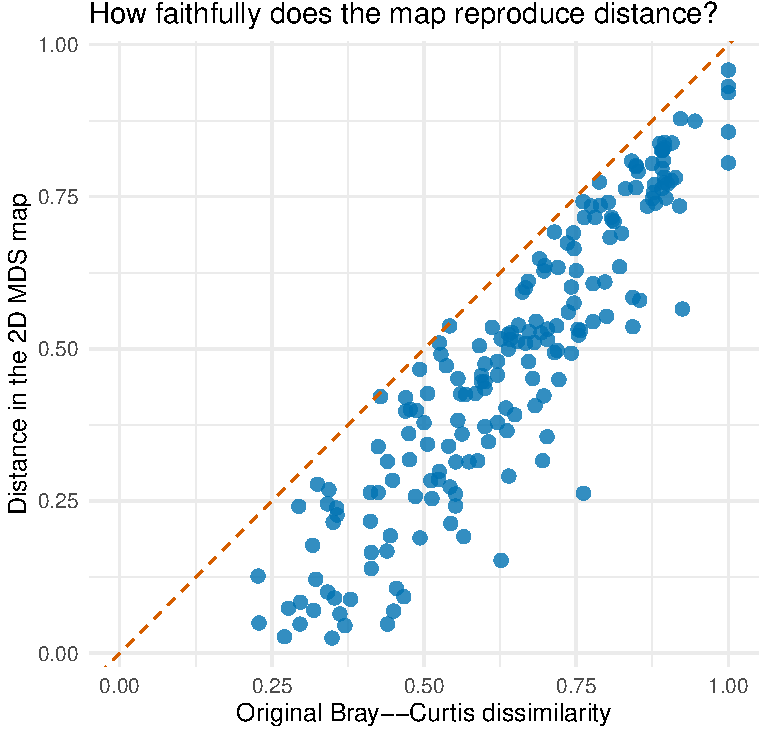
\includegraphics{11_mds_distances_files/figure-latex/shepard-plot-1} 

}

\caption{A Shepard-style plot compares original Bray--Curtis dissimilarities with distances on the two-dimensional MDS map. Points close to the diagonal would indicate perfect reproduction.}\label{fig:shepard-plot}
\end{figure}

\section{Classical MDS and non-metric
MDS}\label{classical-mds-and-non-metric-mds}

Classical MDS tries to preserve the numerical values of distances. If
only the rank order of dissimilarities is trusted, \textbf{non-metric
MDS} is often preferable: it seeks a configuration whose map distances
have the same ordering as the input dissimilarities. Non-metric MDS is
especially common with ecological or ordinal dissimilarities, and is
normally assessed with stress and repeated starts.

We postpone non-metric MDS implementation until students are comfortable
with the classical construction. The conceptual contrast is important:

{\def\LTcaptype{none} % do not increment counter
\begin{longtable}[]{@{}
  >{\raggedright\arraybackslash}p{(\linewidth - 4\tabcolsep) * \real{0.3333}}
  >{\raggedright\arraybackslash}p{(\linewidth - 4\tabcolsep) * \real{0.3333}}
  >{\raggedright\arraybackslash}p{(\linewidth - 4\tabcolsep) * \real{0.3333}}@{}}
\toprule\noalign{}
\begin{minipage}[b]{\linewidth}\raggedright
Method
\end{minipage} & \begin{minipage}[b]{\linewidth}\raggedright
Main aim
\end{minipage} & \begin{minipage}[b]{\linewidth}\raggedright
Diagnostic
\end{minipage} \\
\midrule\noalign{}
\endhead
\bottomrule\noalign{}
\endlastfoot
Classical MDS & Preserve numerical distances as closely as possible &
eigenvalues, distance-reproduction plot \\
Non-metric MDS & Preserve rank order of dissimilarities & stress,
distance-rank plot, stability across starts \\
\end{longtable}
}

\section{Practical workflow}\label{practical-workflow}

When building a distance-based visualization, document these decisions:

\begin{enumerate}
\def\labelenumi{\arabic{enumi}.}
\tightlist
\item
  What are the objects? What are the variables or features?
\item
  Have variables been transformed, standardised or weighted? Why?
\item
  Which distance was chosen, and what kind of difference does it
  represent?
\item
  Does a two-dimensional map reproduce the distances adequately?
\item
  Are map labels and graphical encodings accessible and interpretable?
\item
  Which conclusion is descriptive, and which would require additional
  design or modelling assumptions?
\end{enumerate}

\section{Take-home messages}\label{take-home-messages}

\begin{itemize}
\tightlist
\item
  A distance is a model of what it means for two objects to differ.
\item
  Standardisation is not a neutral default; it changes that model.
\item
  Classical MDS is spectral decomposition applied to a double-centred
  squared distance matrix.
\item
  MDS axes are arbitrary up to rotation and reflection. Interpret
  distances, neighbourhoods and separation instead.
\item
  Negative eigenvalues are informative diagnostics for non-Euclidean
  distances.
\item
  A beautiful MDS map is not sufficient evidence: report the input
  distance and inspect its reproduction.
\end{itemize}

\begin{center}\rule{0.5\linewidth}{0.5pt}\end{center}

\begin{quote}
\textbf{Note on AI assistance}

These teaching materials were prepared with assistance from ChatGPT
(OpenAI) in drafting explanations, developing examples and generating R
code. The author retains responsibility for the final content.
\end{quote}

\end{document}
